\documentclass[]{article}

% Packages

% Pseudocode
\usepackage{algpseudocode}
\usepackage{algorithm}
\usepackage{arrayjob}

% Placing
\usepackage{float}
% Drawing
\usepackage{tikz}
\usetikzlibrary{arrows.meta,chains,%
	decorations.pathreplacing}
% Memory maps
\usepackage{bytefield}
% Simple trees
\usepackage{qtree}
% Better trees
\usepackage{forest} 
% Custom colors
\usepackage{xcolor}
% Comments
\usepackage{verbatim}
% math symbols
\usepackage{amssymb}
% csv reader
\usepackage{csvsimple}
% create file content
\usepackage{filecontents}
% Create c++ fields
\usepackage{listings}
% better tables
\usepackage{tabularx}
\usepackage{graphicx}
\usepackage{caption}
\usepackage{subcaption}
%control
\usepackage{ifthen}

% Plots
\usepackage{pgfplots}
\pgfplotsset{compat = newest}
\usepgfplotslibrary{fillbetween}

% Dependencies
\usepackage{mymacros}
\usepackage{parallelP}

\lstset { %
    backgroundcolor=\color{black!5}, % set backgroundcolor
    basicstyle=\footnotesize,% basic font setting
    numbers=left,                    % where to put the line-numbers; possible values are (none, left, right)
    numbersep=5pt,                   % how far the line-numbers are from the code
    numberstyle=\tiny\color{black}, % the style that is used for the line-numbers
    rulecolor=\color{black},
    keywordstyle=\color{blue},
    tabsize=3,	
}


% Title
\title{Orthogonal Recursive Bisection on the GPU for Accelerated Load Balancing in Large N-Body Simulations \\ - \\ Bachelor Thesis}

\author{Andrin Rehmann}

% Start
\begin{document}

\maketitle

\newpage

\tableofcontents

\newpage
\section{Introduction}

The N-Body technique has been used for decades to simulate the Universe so we can compare theory with observations. This technique uses ``particles'' representing object such as planets and stars. As gravity operates over infinite distance it is necessary to consider all pair-wise interactions which makes a naive implementation $\mathcal{O}(n^2)$.
It is clear that this does not scale particularly well with large particle counts.


One common approach is to partition the space, in which the particles are contained, into a set of subspaces, also called cells, which are then stored in a tree data structure. The process of doing so is very similar to a k-d tree construction. However in our case, where we use a Orthogonal Recursive Bisection (ORB), we do not periodically switch between the individual axes when searching for a median. Instead we pick the axis in which the cell is largest, and search for a median in the particle positions of this axis. The resulting tree is then considered a space partitioning data structure and can be leveraged to perform a multipole expansions of each cell or subspace to approximate the forces acting between the particles. A mutlipole expansion is essentially a mathematical represnation of a group of objects into a single function, we discuss this in further detail later.
This reduces the complexity of the algorithm to $\mathcal{O}(n\log{}n)$. More recently the Fast Multipole Method (FMM), also relying on the space partitioning data structure, has gained wider adoption. This technique further reduces the complexity to $\mathcal{O}(n)$. 

Knowing this we can split the computational effort required in modern N-Body simulations into three categories:

\begin{enumerate}
	\item \textbf{Load Balancing:} In supercomputers we need to distribute the particles equally among computing nodes to make use of the full processing capacity. This needs to be done using ORB in order for us to be able to leverage FFM.
	\item \textbf{Tree Building:} ORB is used again on each node individually to build the fast multipole expansion.
	\item \textbf{Force Calculation and Integration:} We can then leverage the tree on a local and global level combined with FFM to integrate the forces between the particles.
\end{enumerate}

Note that after each time step, the particles have new positions and therefore the space partitioning tree needs to be recomputed as well.

Before the implementation of FMM into codes, and particularly before the era of modern accelerated computing (e.g., SIMD vectorization and GPU computing) the forces calculations (3.) dominated the computational cost. In more recent simulations, each category is about one third of the total calculation time\cite{2017ComAC...4....2P}. This makes the tree building (2.) and load balancing (1.) subjects to great performance gains, since GPU acceleration is usually not exploited. Tree walking and building algorithms heavily rely on control statements such as if / else. SIMD programming in contrast, benefits from large packable data arrays without any branch divergence. Therefore porting tree building code onto the GPU is no easy task and we aim to explore the possibilities and limitations.

We propose to implement tree building on the GPU using CUDA to accelerate load balancing. We will consider implementing the same method for tree building in the future, but set the main target for load balancing.

\subsection{Load Balancing Procedure Overview}

Load balancing is crucial to simulations, because supercomputers with node counts going in the thousands are used for accelerating the runtime. Therefore in an initial step we need to distribute all the particles among the computing nodes in the super computer. To do this randomly, would be very ineffective because we could not make use of FFM anymore. Therefore we apply ORB until we end up with a number of subspaces equivalent to the number of nodes in the system. As we have already mentioned the steps have to repeated after the positions are recomputed, parts of the tree may be preserved as some error is allowed. There may be particles which have moved over the original cell boundaries, but this is acceptable to some level. However we will not focus on updating the data structure and rather assume a complete rebuild after each time step.

The individual steps used for load balancing are as follows:

\begin{enumerate}
	\item 
	The simulation data is stored on a storage device. It contains information about the particles position and further properties.
	
	\pgfmathsetseed{10}
	\begin{figure}[H]
		\begin{center}
			\begin{tikzpicture}
				\foreach \i in {1,...,80}{
					\filldraw [red] (rnd*\linewidth*0.5,rnd*\linewidth*0.5) circle (1pt) node [anchor=west]{};
				}
				\draw (0,0) rectangle (\linewidth*0.5, \linewidth*0.5);
			\end{tikzpicture}
		\end{center}
		\caption{Initial data with particles}
	\end{figure}
	\item
	Since the data is initially unstructured, we distribute it randomly among the nodes in the super computer.
	\pgfmathsetseed{10}
	\begin{figure}[H]
		\begin{center}
			\foreach \j in {1,...,4}{
				\begin{minipage}[c]{0.2\linewidth}
					\begin{tikzpicture}
						\foreach \i in {1,...,20}{
							\filldraw [red] (rnd*\linewidth,rnd*\linewidth) circle (1pt) node [anchor=west]{};
						}
						\draw (0,0) rectangle (\linewidth, \linewidth);
					\end{tikzpicture}
				\end{minipage}
			}
		\end{center}
		\caption{Particles are randomly distributed among 4 nodes}
	\end{figure}
	\item
	We then compute the space partitioning tree data structure with ORB. The datastructure is computed globally across all nodes, meaning that the actual cut positions are the same for all nodes.
	\pgfmathsetseed{10}
	\begin{figure}[H]
		\begin{center}
			\foreach \j in {1,...,4}{
				\begin{minipage}[c]{0.2\linewidth}
					\begin{tikzpicture}
						\foreach \i in {1,...,20}{
							\filldraw [red] (rnd*\linewidth,rnd*\linewidth) circle (1pt) node [anchor=west]{};
						}
						\draw (0,0) rectangle (\linewidth, \linewidth);
						
						\draw (0,0) rectangle (\linewidth*0.55, \linewidth);
						
						\draw (0,0) rectangle (\linewidth*0.55, \linewidth*0.6);
						
						\draw (\linewidth*0.55,0) rectangle (\linewidth, \linewidth*0.5);
						
					\end{tikzpicture}
				\end{minipage}
			}
		\end{center}
		\caption{Space partitioning tree data structure is computed}
	\end{figure}
	
	\item
	In a final step we distribute the particles among the nodes in way such that each node only owns particles within a leaf node of the space partitioning tree data structure.
	\begin{figure}[H]
		\begin{center}
			\pgfmathsetseed{10}
			\begin{minipage}[c]{0.2\linewidth}
				\begin{tikzpicture}
					\foreach \i in {1,...,80}{
						\filldraw [red] (rnd*\linewidth,rnd*\linewidth) circle (1pt) node [anchor=west]{};
					}
					\draw[fill=white] (0,0) rectangle (\linewidth*0.55,  \linewidth*0.6);
					\draw[fill=white] (\linewidth*0.55,0) rectangle (\linewidth,  \linewidth*0.5);
					\draw[fill=white] (0,\linewidth*0.6) rectangle (\linewidth*0.55,  \linewidth);
					\draw (\linewidth*0.55,\linewidth*0.5) rectangle (\linewidth,  \linewidth);
					
				\end{tikzpicture}
			\end{minipage}
			\pgfmathsetseed{10}
			\begin{minipage}[c]{0.2\linewidth}
				\begin{tikzpicture}
					\foreach \i in {1,...,80}{
						\filldraw [red] (rnd*\linewidth,rnd*\linewidth) circle (1pt) node [anchor=west]{};
					}
					\draw[fill=white] (0,0) rectangle (\linewidth*0.55,  \linewidth*0.6);
					\draw[fill=white] (\linewidth*0.55,0) rectangle (\linewidth,  \linewidth*0.5);
					\draw (0,\linewidth*0.6) rectangle (\linewidth*0.55,  \linewidth);
					\draw[fill=white] (\linewidth*0.55,\linewidth*0.5) rectangle (\linewidth,  \linewidth);
					
				\end{tikzpicture}
			\end{minipage}
			\pgfmathsetseed{10}
			\begin{minipage}[c]{0.2\linewidth}
				\begin{tikzpicture}
					\foreach \i in {1,...,80}{
						\filldraw [red] (rnd*\linewidth,rnd*\linewidth) circle (1pt) node [anchor=west]{};
					}
					\draw[fill=white] (0,0) rectangle (\linewidth*0.55,  \linewidth*0.6);
					\draw (\linewidth*0.55,0) rectangle (\linewidth,  \linewidth*0.5);
					\draw[fill=white] (0,\linewidth*0.6) rectangle (\linewidth*0.55,  \linewidth);
					\draw[fill=white] (\linewidth*0.55,\linewidth*0.5) rectangle (\linewidth,  \linewidth);
				\end{tikzpicture}
			\end{minipage}	
			\pgfmathsetseed{10}
			\begin{minipage}[c]{0.2\linewidth}
				\begin{tikzpicture}
					\foreach \i in {1,...,80}{
						\filldraw [red] (rnd*\linewidth,rnd*\linewidth) circle (1pt) node [anchor=west]{};
					}
					\draw (0,0) rectangle (\linewidth*0.55,  \linewidth*0.6);
					\draw[fill=white] (\linewidth*0.55,0) rectangle (\linewidth,  \linewidth*0.5);
					\draw[fill=white] (0,\linewidth*0.6) rectangle (\linewidth*0.55,  \linewidth);
					\draw[fill=white] (\linewidth*0.55,\linewidth*0.5) rectangle (\linewidth,  \linewidth);
				\end{tikzpicture}
			\end{minipage}
		\end{center}
		\caption{Leaf cells of data structure are distributed among nodes}
	\end{figure}
\end{enumerate}

\begin{comment}
\subsection{Force Integration}


\begin{figure}[H]
	\begin{center}
		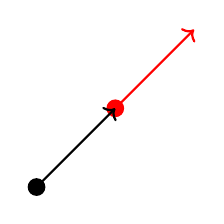
\begin{tikzpicture}
			\filldraw  (0,0) circle (3pt) node [anchor=west]{};
			\filldraw[red]  (1,1) circle (3pt) node [anchor=west]{};
			\draw[->, thick] (0,0) -- (1,1);
			\draw[->, red, thick] (1,1) -- (2,2);
		\end{tikzpicture}
	\end{center}
\end{figure}
\end{comment}

\subsection{Fast Multipole Expansion}

A multipole expansion can be used to approximate a function. In our case, we aim to approximate the gravity field of the particles contained within a cell. This simplification of gravitational fields is used to group particles together such that the group can be treated as a single object. 

For an intuitive understanding, one can imagine a large cluster of particles that is very far away from planet Earth. If we wish to compute the interactions between every single object of the cluster and Earth, we will need to perform $O(n^2)$ computations. However, since the object is reasonably far away, it does not make sense to compute every interaction. Instead, we summarize the cluster into a single object, which is represented as a function. We can then simply compute the interacting gravity between planet Earth and the function. Since we are bound by numerical accuracy anyways, the error term introduced by simplifying calculations with the fast multipole method can also be kept so small that it does not exceed the numerical error. Consequently, objects within our own solar system would be too close to planet Earth to approximate its effects using a multipole. In such cases, it is necessary to perform all $O(n^2)$ computations.

After we have built the space partitioning tree, we compute the multipole for all cells in the tree. This allows us to dynamically select more or less detailed functions to represent a group of particles. Depending on the distance between the particle we want to determine the forces for and the particles which exert the forces, we might choose a higher or lower multipole expansion.

As we have mentioned, when using ORB to create the space partitioning tree data structure, we always search for a median in the axis where the cell size is largest. This is the best method to avoid skewed shapes and approximate squarish shapes. 

As described in \cite{Stadel2001}, "the opening radius of a cell is given by some constant factor times $r_{max}$". $r_{max}$ is the distance between the center of mass of a cell and its most distant corner. The opening radius correlates with the error ratio, which in turn influences how fine grained the timesteps many calculations have to be performed. Trivially, a square is the rectangle where the distance between any point and its most distant corner point is the smallest. Thus, we will want to approach more square-like shapes.

The most straight forward way to avoid high ratios between the length and height of such a rectangle is to always split it along its longest axis.

\subsection{Target Data and Notation}\label{section:target-data}

The target data consists of $N$ particles where we use the following notations:

\begin{itemize}
	\item We define a particle as $par_i$  where $i \in \{0,...,N\}$. 
	\item We define the space of binary numbers with a precision of $p$ as $\mathbb{B}_p$ where we have $a \in \mathbb{B}_p \Leftrightarrow a \in \{0,1\}^{p}$
	\item We define the corner coordinates of root domain with $\vec{lower}, \vec{upper}$ where we have $\vec{lower}, \vec{upper} \in \mathbb{B}_p^3$. 
	\item We define the coordinates of a particle $par_i$ as $\vec{x_i}$ for which holds $\{\vec{x} | \vec{lower} \leq \vec{x} \leq \vec{upper}, \vec{x} \in \mathbb{B}_p^3 \}$.
	When refering to a single coordinate of a particle object we do so by writing $\vec{x}_{i,j}$. Finally the array of all particles positions in a single axis is denoted as $\vec{x}_{:,j}$. 

\end{itemize}

The distribution of the entire dataset cannot easily be characterized. There may be areas with very dense distribution, separated by vastly unpopulated areas. Thus it is best to make no assumptions about the dataset and expect anything.

\begin{figure}[H]
	\begin{center}
		\begin{tikzpicture}
			\randistr{10}{5}{100}
			\draw (0,0) rectangle (10, 5);
			\filldraw  (0,0) circle (3pt) node [anchor=west]{};
			\node[yshift=0.3cm, xshift=-0.3cm] at (0,0) {$-\frac{b}{2}$};
			
			\filldraw  (10,5) circle (3pt) node [anchor=west]{};
			\node[yshift=0.3cm, xshift=-0.3cm] at (10,5) {$\frac{b}{2}$};
		\end{tikzpicture}
	\end{center}
\caption{Uniform random distribution of 3D coordinates in cube domain projected onto a 2d plane}
\end{figure}

\subsection{PKDGrav}

\subsection{Ralated Work}

\TODO{Write how ORB is similar to quicksort, how individual parts could be done using thrust library.}
\newpage
\section{Orthogonal Recursive Bisection (ORB)} \label{section:orb}


%https://de.overleaf.com/learn/latex/TikZ_package
%https://texample.net/tikz/examples/
The ORB algorithm partitions a multi-dimensional domain into subdomains based on spatial proximity, by splitting a $k$-dimensional domain containing $N$ particles into $d$ subdomains each of $k$ dimensions. This can be done using a recusive process where all intermediate domains are stored in a binary tree. A node of this tree is referred to as a $cell$. A $cell$ is a datastructure which keeps track of the domain information and also keeps pointers to its two child cells. The final binary tree should have exactly $d$ leaf cells. 

Our main objective in this work is to improve the runtime of astrophysical simulations, or more specifically PKDGrav. At the same time we want to minimize penalties with regards to $N$, the total number of particles, such that we can leverage a high $N$ to increase the precision of the simulation. Furthermore we want to adapt and optimize the algorithms with regards to the target data as introduced in \ref{section:target-data} and target computing systems (\ref{section:target-systems}).

\subsection{By example} 
For the purpose of explaining the algorithm both visually and by a numeric example, we consider the following minimal dataset:

\begin{filecontents*}{particles10.csv}
x,y,id,o1,o2,x2,y2
0.4,0.3,0,0,0,0.4,0.3
0.2,0.6,1,2,1,0.2,0.6
0.8,0.9,2,1,2,0.9,0.8
0.6,0.5,3,0,0,0.6,0.5
0.3,0.8,4,1,1,0.3,0.8
0.7,0.1,5,2,2,0.7,0.1
0.9,0.3,6,2,2,0.9,0.3
\end{filecontents*}

\begin{filecontents*}{particles11.csv}
	x,y,id
	0.4,0.3,0
	0.2,0.6,1
	0.3,0.8,4
	0.6,0.5,3
	0.8,0.9,2
	0.7,0.1,5
	0.9,0.3,6
\end{filecontents*}


\begin{filecontents*}{particles12.csv}
	x,y,id
	0.4,0.3,0
	0.6,0.5,3
	0.3,0.8,4
	0.2,0.6,1
	0.8,0.9,2
	0.7,0.1,5
	0.9,0.3,6
\end{filecontents*}

\begin{figure}[H]
    \begin{center}
        \begin{minipage}[c]{0.2\linewidth}
        \csvreader[
            tabular=ccc,
            table head=\hline \bfseries{x} & \bfseries{y} & \bfseries{id} \\\hline,
            late after last line=\\\hline % horizontal line at the end of the table
            ]{particles10.csv}{}{\csvcoli & \csvcolii & \csvcoliii}
        \end{minipage}
        \begin{minipage}[c]{0.7\linewidth}
            \begin{tikzpicture}
                \begin{axis}
                 [
                    nodes near coords,
                    xmin=0,
                    xmax=1,
                    ymin=0,
                    ymax=1
                ]
                \addplot+[
                    only marks,
                    point meta=explicit symbolic
                ] table [
                    x=x, 
                    y=y, 
                    meta=id, 
                    col sep=comma] 
                {particles10.csv};
                \end{axis}

            \end{tikzpicture}
        \end{minipage}
    \end{center}
\caption{Example distribution with $N$ = 7}
\end{figure}


\subsection{Memory and Workload Balancing}\label{balancing}
We have now formulated our main objectives for improving ORB, which are (1) to improve the runtime, which is done with workload balancing, whilst (2) at the same time keeping $N$ as large as possible. In this section we will explain the averse effects when disregarding interactions between minimizing runtime and maximizing N.

\Q{Is N fixed? simulated?}


If we want to reduce the error of the force integration across all particles, we need to introduce more discrete time steps for certain particles than for others. The need for non-constant simulations steps across the simulation is caused by the vastly variant forces which are exercised on different particles. It is possible that certain particles follow a straight path with an almost constant velocity, whereas others are influenced by strong gravitational poles. 

We denote the workload for a particle $p_i$ as the weighting function $w(p_i)$. The workload correlates with the number of simulations steps, that need to be computed for a single particle. In an optimally parallelized system, the workload should be very similar among computing units, thus it would make sense to distribute the particles regarding the weighting function. This in turn implies an unequal distribution of the particles with regards to memory.

Let us consider a simple example to illustrate the point. Given the set of particles $A = \{p_1, p_2, .., p_{2m/3}\}$ and respectively $B = \{p_{2m/3 + 1}, p_2, .., p_{m}\}$. This gives us a total number of particles equivalent to $N = m$. Let us now consider that $\forall p \in A : w(p) = 1$ and $\forall p \in B : w(p) = 2$. If we assign all particles from set $A$ to process with rank 0 and the particles from B to rank 1. It is clear that $\sum_{p\in A} w(p) = \sum_{p\in B} w(p)$. Thus the two processors are balanced in terms of computing costs, but clearly they are not balanced in terms of memory size. In fact, process with rank 0 has $2m/3$ elements and rank 1 has $m/3$ elements. Assuming each process has a memory size of $2m/3$, then clearly this configuration is not optimal. If we were to favor memory balancing, we could assign $2m/3$ to each processor and we would be able process $(4/3) \times m$ particles in total, which is larger than the original $N$ and therefore favorable.

To which degree we decide to favor memory over workload balancing is difficult to answer. But as for now we will parametrize the workload using the weighting function, which allows us to optimize and decide at a later stage. If we decide to completely ignore the workload balancing and solely focus on memory balancing, we can simply set the $w(p_i) = 1$ for all particles.


\subsection{ORB}


In each recursive call of the ORB algorithm, we are given a $cell$ along with a number of desired leaf cells $d_{cell}$, which corresponds to $d$ for the root cell. Furthermore each cell has information about the volume it encompasses (also refereed to its domain) stored as $V_{cell}$. We then split this $cell$, into two child cells $leftCell$ and $rightCell$. For the domains of $leftCell$ and $rightCell$ we have the following properties: 

\begin{center}
	\begin{equation}
		V_{cell} = V_{leftCell} \cup V_{rightChild}
	\end{equation}
\end{center}

\begin{center}
	\begin{equation}
		V_{leftCell} \cap V_{rightChild} = \emptyset
	\end{equation}
\end{center}

How the volumes of the child cells are exactly defined, will be explained in later stages of this section. Primarily we need to define the variable $d$ for the child cells.

Given a cell, we recursively define $nLeafCells$ for its children as follows:

\begin{center}
	\begin{equation}
		d_{leftCell} = \left \lceil\frac{d_{cell}}{2} \right \rceil 
	\end{equation}
\end{center}

\begin{center}
	\begin{equation}
		d_{rightCell} = d_{cell} - d_{leftCell}
	\end{equation}
\end{center}

Finally we need to determine the number of particles, which should be encompassed in $V_{leftCell}$ and $V_{rigtCell}$. We define the number of particles in the current cell as $N_{cell}$, respectively the left and right child cells are defined as follows:

\begin{center}
	\begin{equation}
		N_{leftCell} = min \left \{ x \in \{0,...,N_{cell} \} : \sum_{i=0}^{x} w(p_i) \geq \frac{d_{leftCell}}{d_{cell}} \times \sum_{i=0}^{N_{cell}} w(p_i) \right \} 
	\end{equation}
\end{center}

\begin{center}
	\begin{equation}
		N_{rightCell} = N_{cell} - N_{leftCell}
	\end{equation}
\end{center}

With this formula we make sure, that for any given $d$, we can subdivide the domain accordingly and end up with leaf cells, who encompass an almost equal amount of particles.


To simplify the visual and numeric explanation of the ORB algorithm, we assume $\forall i \in \{0,..,N\} : w(p_i) = 1$.

The ORB algorithm is initiated by considering the volume $V_{cell}$ which encompasses all particle coordinates. In each iteration we use a binary search algorithm, which we will introduce in later stages, to determine a cut $c$ position. This cut position is defined along a specified axis, which is determined by the dimension where the domain is largest. In three dimensional space we can then represent this cut as a plane and make simple checks weather a particle is right or left of this plane. 

The ideal cut plane is defined such that exactly $N_{leftChild}$ particles are located to its left side. This cut plane allows us to split the volume $V_{cell}$ in two subdomain, where the $V_{leftCell}$ is constrained by our original domain boundaries and the cut plane on its right side. The same can be done for the right cell, where the cut plane determines the left side boundaries of the volume $V_{rightCell}$. We repeat this process until we have segmented our initial domain into $d$ leaf cells.


    
\begin{figure}[H]

        \centering
            \begin{tikzpicture}
                \begin{axis}
                [
                    nodes near coords,
                    xmin=-0.,
                    xmax=1.,
                    ymin=-0.,
                    ymax=1.,
                ]
                \addplot    +[
                    only marks,
                    point meta=explicit symbolic
                ] table [
                    x=x, 
                    y=y, 
                    meta=id, 
                    col sep=comma] 
                {particles10.csv};
                \draw [fill=red!20](0.0,0.0) rectangle (1, 1);
                \node[below] at (0.5, 1){$cell_1$};
                \end{axis}
            \end{tikzpicture}
\caption{Example particles with ORB at recursion depth 0}
\label{fig:orb1}
\end{figure}

\begin{figure}[H]
    \centering
    \begin{forest}
        [$cell_1$
        []  
        ]
    \end{forest}    
\caption{Tree with ORB at recursion depth 0}
\end{figure}

\begin{figure}[H]
	\begin{center}
		\begin{tikzpicture}
			\pgfmathsetseed{2};
                \begin{axis}
                [
                    nodes near coords,
                    xmin=-0.,
                    xmax=1.,
                    ymin=-0.,
                    ymax=1.,
                ]
                \addplot+[
                    only marks,
                    point meta=explicit symbolic
                ] table [
                    x=x, 
                    y=y, 
                    meta=id, 
                    col sep=comma] 
                {particles10.csv};
                \draw [fill=green!20](0.0,0.0) rectangle (0.65, 1);
                \draw [fill=blue!20](0.65,0.0) rectangle (1, 1);
                \node[below] at (0.2, 1){$cell_2$};
                 \node[below] at (0.7, 1){$cell_3$};
                \end{axis}
            
		\end{tikzpicture}
    \end{center}
\caption{Example particles with ORB at recursion depth 1}
\label{fig:orb2}
\end{figure}

\begin{figure}[H]
\centering
	\begin{forest}
		[$cell_1$
		[$cell_2$][$cell_3$]  
		]
	\end{forest}    
\caption{Tree with ORB at recursion depth 1}
\end{figure}

\begin{figure}[H]
	\begin{center}
		\begin{tikzpicture}
			\pgfmathsetseed{2};
                \begin{axis}
                [
                    nodes near coords,
                    xmin=-0.,
                    xmax=1.,
                    ymin=-0.,
                    ymax=1.,
                    title=Recursion depth 2
                ]
                \addplot+[
                    only marks,
                    point meta=explicit symbolic
                ] table [
                    x=x, 
                    y=y, 
                    meta=id, 
                    col sep=comma] 
                {particles10.csv};
                \draw [fill=pink!20](0.0,0.0) rectangle (0.65, 0.55);
                \draw [fill=yellow!20](0.0,0.55) rectangle (0.65, 1);
                \draw [fill=blue!20](0.65,0.0) rectangle (1, 1);
                \node[below] at (0.2, 1){$cell_4$};
                \node[above] at (0.2, 0){$cell_5$};
                \node[below] at (0.7, 1){$cell_3$};
                \end{axis}
            
		\end{tikzpicture}
    \end{center}
\caption{Example particles with ORB at recursion depth 2}
\label{fig:orb3}
\end{figure}

\begin{figure}[H]
	\centering
	\begin{forest}
		[$cell_1$
		[$cell_2$ [$cell_4$] [$cell_5$]][$cell_3$]  
		]
	\end{forest}
 \caption{Tree with ORB at recursion depth 2}
\end{figure}


Since $d_{cellLeft} - d_{cellRight}$ must always be $\leq 1$, it must hold that the tree is a nearly complete binary tree. Therefore we can conclude that the height of the tree is equal to $\lceil log(d) \rceil$ and the total number of nodes (not only leaf nodes) is $log(d) \times d$. Since we have a nearly complete binary tree, we also have the possibility of storing it in a heap data-structure, which can in turn greatly increase the performance, since we will not have to perform a tree walk to access individual cells in the tree.

\Q{Cant we assume for the reader to know what a heap is?}
\begin{figure}
	
	\begin{algorithm}[H]
		\caption{The ORB main routine}\label{euclid}
		\begin{algorithmic}[1]
			\Procedure{orb}{$\vec{lower}, \vec{upper}, d$}
			\State $\vec{size} = \vec{upper} - \vec{lower}$
			\State $i = maxIndex(\vec{size}_0, \vec{size}_1, \vec{size}_2)$ \Comment{Get index of max value}
			\newline
			\State $d^\prime_{i \times 2 } = \left \lceil\frac{d}{2} \right \rceil$
			
			\State $cut = cut(\vec{lower}_{i}, \vec{upper}_{i}, i, \frac{d^\prime}{d} )$
			\State $mid = partition(split, axis)$
			\newline
			
			\State $\vec{upper^\prime} = \vec{upper}$
			\State $upperChild_{i} = cut$
			\State $\vec{lower^\prime} = \vec{lower}$
			\State $lowerChild_{i} = cut$
			\newline
			
			\State \Call{orb}{$\vec{lower}, \vec{upper^\prime}, d^\prime $}
			\State \Call{orb}{$\vec{lower^\prime}, \vec{upper}, d - d^\prime $}
			\EndProcedure
		\end{algorithmic}
	\end{algorithm}
\label{proc:orb}
\end{figure}

Let not apply the algorithm to our running example:

\TODO{Insert step by step algorithm here}

\subsection{Root finding}


%Finding the median of a large particle array is an essential step for ORB. We will thus explore different algorithms alongside their advantages and disadvantages for our specific use case.
%Note that there exists approximation algorithms for example the median of medians algorithms. But the correctness guarantee of the median lying between 30\% and 70\% is not good enough in our case. If we were to implement such an approximation algorithms we would run into similar issues as described in \ref{sec:balancing}. But in this case the unequal memory balancing do not have the advantage of equal workload balancing, which in turn will worsen the performance and the maximum number of workable particles. Thus we will only consider approximation algorithms, if their approximation to the ideal values are very exact and can be determined.

 The $cut$ algorithm takes an array of particles, an axis, a left and right boundary as well as a percentage $r$ of particles which should be on the left side to the determined cut. Its goal is to return a position, such that the particles on the left side of the cut are equal to the percentage input parameter multiplied by all particles. We can define a function $f(c)$ where the function evaluates the number of elements smaller than the cut value c minus half the number of total particles. Reformulated in this way, the problem is equivalent to a root finding problem. Because when the function evaluates to zero, we have found a cut plane positions where exactly half the particles are located to left side. There exists a lot of different solver for the root finding problem, the most stable and easiest to implement is however the bisection method.
 
 Since we are operating on binary numbers with a limited precision, the bisection method is guaranteed to terminate after a certain number of steps. Other approximate algorithms can converge quicker, meaning they find the root in less time steps, than the bisection method, however they are not guaranteed to converge.

\subsubsection{Bisection Method}

The first step is to make an estimation for a cut. In our case we simply assume it to be the exact middle of the domain boundaries. In principle the binary cut counts the number of particles on the left side of the of an initial cut. In case the particles are less than half of all particles, its clear that the cut was too far to the left, and the new right boundary of the domain is the cut. In case the particles are more than half, we set the the left boundary as the cut. This is repeated until we find a precise cut position.


\begin{figure}
	
	\begin{algorithm}[H]
		\caption{Bisection Method}\label{algo:cut}
		\begin{algorithmic}[1]
			\Procedure{cut}{$left, right, axis, percentage$}
			\State $nLeft = 0$
			\State $cut = 0$
			\newline
			\For{$k \in {0,..,p}$}
			\State $cut = (right + left ) / 2 $
			\State $nLeft\gets sum(x_{:,axis} < cut)$
			\newline
			\If{$abs(nLeft - N_j) * percentage< \alpha $}
			\State Break
			\EndIf
			\newline
			
			\If{$nLeft <= N_j * percentage$}
			\State $left = cut$
			\Else 
			\State $right = cut$
			\EndIf
			\newline
			\EndFor
			\State \Return $cut$
			\EndProcedure
		\end{algorithmic}
	\end{algorithm}
\caption{Bisection Method}
\label{proc:cut}
\end{figure}


\subsubsection{Edge cases}

Let us consider the following example particle distribution where $particle_1$ and $particle_2$ have identical x coordinates. 

\begin{figure}[H]
	\begin{center}
		\begin{tikzpicture}
			\draw [ dashed](5 cm, 0 cm) -- (5 cm, 3 cm);
			\cutoffdistr{10}{3}{3};
			\draw (0,0) rectangle (10, 3);
		\end{tikzpicture}
	\end{center}
\end{figure}

If we want to split this domain, there would not exists a correct split, where $nLeft$ is equal to $\frac{N}{2}$. In fact this example can be made more extreme by adding more particles which are distributed along a the line.
The $\alpha$ value defines by how many particles the final cut value can be off from the actual ideal median value. In this case we would assign $particle_0$ to the left child cell and the other particles to the right child cell. Since we have seen that there exists counter examples, where no optimal solution can be found, with a reasonably small $\alpha$ we add another break condition which is fulfilled after 32 iterations. If no solution has been found after that many iterations, it is clear that we cannot improve the cut anymore, because we have reached the precision limit.

\subsubsection{Runtime Analysis}

We analyse the runtime of the cut algorithm as follows: On line 5 we count the number of particles on the left side of the cut position. Since the array is unordered, we need to sweep over all the elements once which results in a runtime of $O(N)$. All other operartions inside the for loop can be computed in a negligible constant time. The loop itself is repeated $p$ number of times, where $p$ corresponds to the precision of the array data. With each iteration we half the span in which the optimal solution lies. Thus we reach the precision limit after $p$ iterations. Note that due to the Break condition on line 7, the average runtime is not the same as the maximum runtime and depends a lot on the underlying data.

The bisection method converges rather slowly, \TODO{Explain} assuming its first guess for the cut position was almost correct, it will correct its next guess by $25\%$ of the entire domain size, thus the number of iterations need to approach the actual optimum again is rather high.  

\begin{comment}

\subsubsection{Binary Search with improved guessing}

As we can see in \ref{algo:cut}, the initial guess of the cut is simply the center of the domain. But if we consider non uniform distributions, this initial guess can possibly rather bad. Let us consider the following example:

\begin{figure}[H]
	\begin{center}
		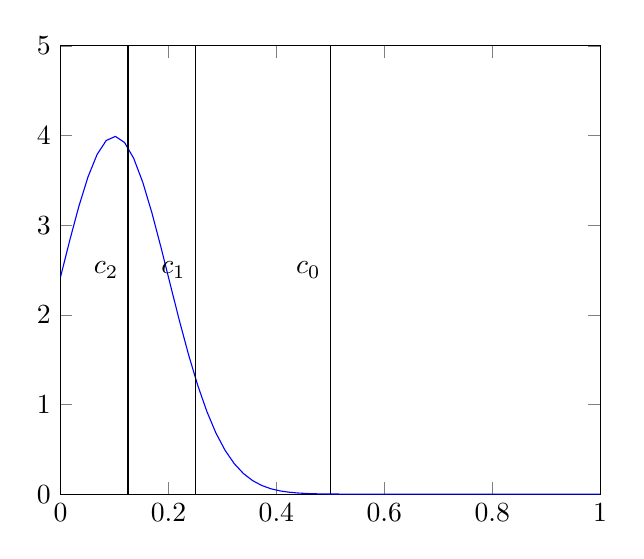
\begin{tikzpicture}
			\def\mean{0.1}
			\def\sigma{0.1}
			\def\pi{3.14159265359}
			\begin{axis}[xmin = 0, xmax = 1, ymin=0, ymax=5, samples=60]
				\addplot[domain = 0:1,blue] {1 / (\sigma * sqrt(2 * \pi)) * exp(-0.5 * ((x - \mean) / \sigma)^2) };
				\draw (axis cs:0.5,0) -- node[left]{$c_0$} (axis cs:0.5,5);
				\draw (axis cs:0.25,0) -- node[left]{$c_1$} (axis cs:0.25,5);
				\draw (axis cs:0.125,0) -- node[left]{$c_2$} (axis cs:0.125,5);
			\end{axis}
		\end{tikzpicture}
	\end{center}
	\caption{3 iterations of binary search with naive initial guess}\label{euclid}
\end{figure}

The underlying distribution is a normal distribution. \TODO{Add reference to section about data}. We can see that the algorithm will have to sweep 3 times over the entire array to get into the region of the actual median. One suggestion for improvement is to use an approximated median as a guess for the first split. We can sample 100 particles and find their median in constant time. Then we will run the binary cut algorithm using the approximated median as an initial guess. This can reduce the runtime by a few iterations, however we cannot make any assessment about the runtime, as this improvement will make the algorithm even slower on some distributions. Let us for example consider the uniform distribution, in this case the addition is pure overhead as the center is already the most accurate initial guess.
\end{comment}



\subsection{Partition Algorithm}

We have already introduced all basic building blocks of the ORB algorithm. The only and final piece which is missing is the partition algorithm. We want to continuously update the array and in the words used before, have a direct correlation between $x_i$ and $i$. This allows us to group all particles, which are contained in a cell in a fixed range of indexes of the particles array. The advantages of this are two fold: Firstly we can access all particles within a cell in constant time, secondly this allows us to easily manipulate particles within a cell as a slice. The disadvantage is a slight increase in runtime which comes with the partitioning algorithm.

When thinking about this in terms of the recursive algorithm, maintaining this data structure is pretty straight forward. Each time we split a cell into two children, we make sure that particles contained in the left child cell are found in a designated range of the particles array, and the exact same concept is applied to the right cell. The partition algorithm is equivalent to the common hoare partition algorithm. \TODO{Add reference}

\TODO{Add explanation}
\begin{algorithm}[H]
	\begin{algorithmic}[1]
		\Procedure{partition}{$x, N_j, cut, axis$}
		\State $i = 0$
		
		\For{$k \in {0,..N_j - 1}$}
		\If{$\vec{x}_{k, axis} < cut$}
		\State $i = i + 1$
		\State $x_{i}, x_{k} = x_{k}, x_{i}$
		\EndIf
		\EndFor
		
		\State $ x_{i}, x_{N_j-1} = x_{N_j-1}, x_{i}$
		\EndProcedure
	\end{algorithmic}
\caption{Partition Method}
\end{algorithm}

The partition algorithm has a clearly observable runtime of $O(N)$ since we iterate over all particles once. Since we need to touch each element at least once to partition the entire array there is no better algorithm than this.

Lets apply the algorithm to our running example. We start with our initial array of particles as follows:

\begin{figure}[H]
	\begin{center}
		\csvreader[
		tabular=ccc,
		table head=\hline \bfseries{x} & \bfseries{y} & \bfseries{id} \\\hline,
		late after last line=\\\hline % horizontal line at the end of the table
		]{particles10.csv}{}{\csvcoli & \csvcolii & \csvcoliii}
	\end{center}
\end{figure}

We then partition the particles with a cut in the x axis set to 0.65 as seen in figure \ref{fig:orb2}.

\begin{figure}[H]
	\begin{center}
		\csvreader[
		tabular=ccc,
		table head=\hline \bfseries{x} & \bfseries{y} & \bfseries{id} \\\hline,
		late after last line=\\\hline % horizontal line at the end of the table
		]{particles11.csv}{}{\csvcoli & \csvcolii & \csvcoliii}
	\end{center}
\end{figure}

Finally we partition $cell_2$ into $cell_4$ and $cell_5$ with the cut position 0.55 along the y axis as seen in figure \ref{fig:orb2}. We end up with the following array:

\begin{figure}[H]
	\begin{center}
		\csvreader[
		tabular=ccc,
		table head=\hline \bfseries{x} & \bfseries{y} & \bfseries{id} \\\hline,
		late after last line=\\\hline % horizontal line at the end of the table
		]{particles12.csv}{}{\csvcoli & \csvcolii & \csvcoliii}
	\end{center}
\end{figure}

Note how all particles from $cell_4$ are contained in the range of 0-1. The particles of $cell_5$ in 2-3 and finally the particles contained in the volume of $cell_3$ can be found in 4-7.

\subsection{Parallelize ORB }\label{sec:parellize-orb}

In the context of parallelization, we define the number of processors as $np$. When the goal of the algorithm is workload balancing, we will want to set $d = np$ to end up with exactly as many leaf cells as we have processors. In the context of a supercomputing system $np$ is usually equivalent to the number of nodes in the system.

Initially we assume that each processor has a random unique subset of all the particles stored in its memory, this has two reasons. For one we run into memory limitations quickly when trying to load all the particles onto a single node, furthermore memory bandwidths limitations can be multiplied by the number of processors and are thus a lot higher. 

Let us now apply this to our running example where we have 3 nodes.

\begin{figure}[H]
	
	\centering
	\begin{tikzpicture}
		\begin{axis}
			[
			nodes near coords,
			xmin=-0.,
			xmax=1.,
			ymin=-0.,
			ymax=1.,
			title=Recursion depth 0,
			legend cell align=left
			]
			
			\addplot    +[
			only marks,
			point meta=explicit symbolic,
			restrict expr to domain={\thisrow{o1}}{0:0}, 
			] table [
			x=x, 
			y=y, 
			meta=id, 
			col sep=comma] 
			{particles10.csv};
			
			\addplot    +[
			only marks,
			point meta=explicit symbolic,
			restrict expr to domain={\thisrow{o1}}{1:1}, 
			] table [
			x=x, 
			y=y, 
			meta=id, 
			col sep=comma] 
			{particles10.csv};
			
			\addplot    +[
			only marks,
			point meta=explicit symbolic,
			restrict expr to domain={\thisrow{o1}}{2:2}, 
			] table [
			x=x, 
			y=y, 
			meta=id, 
			col sep=comma] 
			{particles10.csv};
			
			\legend{$p0$,$p1$,$p3$}
			
			%\draw [fill=red!20](0.0,0.0) rectangle (1, 1);
			%\node[below] at (0.5, 1){$cell_1$};
		\end{axis}
	\end{tikzpicture}
	\caption{Example particles distributed randomly across 3 nodes}
\end{figure}

The ORB algorithm is only executed form the operative node, all other nodes are purely worker nodes and perform certain parts of the algorithm. In our case one of the most performance intensive tasks is found on line 6 from the cut procedure as seen in figure \ref{proc:cut}. Not only is it costly, its also a task that can only be executed from the node, which owns the particles array, i.e. its stored in its memory. Therefore the worker nodes count the number of particles on the left side of a 2D cut plane individually and send back the results to the operative thread as seen in figure \ref{fig:orbp}. Besides the counting we also have the partitioning which also concerns the particles array and thus can only be executed by its corresponding owner. Consequently the procedure is also executed on the worker nodes individually. Note that the operative node can also perform work, thus become a worker node at times. This can be seen in figure \ref{fig:orbp}, where p0 is the operative node, but still performs partition and counting operations.

\begin{figure}[H]
	\begin{center}
		\begin{tikzpicture}
			
			\timeline{6}{16}{3}
			
			
			\parallelloop{-2}{15.5}{8}{0.5}{loop till desired tree depth is reached};
			
			\parallelloop{-1}{11.5}{7}{3.5}{loop till cut found};
			
			\communication{Broadcast cells}{0}{7}{15};
			
			\process{partition}{0}{14};
			\process{partition}{2}{14};
			\process{partition}{4}{14};
			\process{partition}{6}{14};
			
			\process{compute\\ cut}{0}{11};
			
			
			\communication{Broadcast cut from operative}{0}{7}{8};
			
			\process{count \& \\ count left}{0}{7};
			\process{count \& \\ count left}{2}{7};
			\process{count \& \\ count left}{4}{7};
			\process{count \& \\ count left}{6}{7};
			
			
			\communication{Reduce count to operative}{0}{7}{4};
			
			\process{generate\\ new \\ cells}{0}{3};
			
		\end{tikzpicture}
	\end{center}
	\caption{Parallelized ORB for np = 4}
	\label{fig:orbp}
\end{figure}


\begin{comment}
\subsubsection{Global Partitioning}

In the case of global partitioning, we partition the particle in such a way, that we can decouple the left and right child's computations completely from each other. In order to achieve this, the particles need to be redistributed among threads, s.t. each thread contains only particles contained in a single cell. Which in turn means it only need to consider particles in a designated volume. Finally this allows us to run the thread completely independent from others and remove the overhead introduced by synchronization operations.
When looking at the numeric example this might look as follows:


\begin{figure}[ht]
	
	\centering
	\begin{tikzpicture}
		\begin{axis}
			[
			nodes near coords,
			xmin=-0.,
			xmax=1.,
			ymin=-0.,
			ymax=1.,
			title=Recursion depth 0,
			legend cell align=left
			]
			
			\addplot    +[
			only marks,
			point meta=explicit symbolic,
			restrict expr to domain={\thisrow{o1}}{0:0}, 
			] table [
			x=x, 
			y=y, 
			meta=id, 
			col sep=comma] 
			{particles10.csv};
			
			\addplot    +[
			only marks,
			point meta=explicit symbolic,
			restrict expr to domain={\thisrow{o1}}{1:1}, 
			] table [
			x=x, 
			y=y, 
			meta=id, 
			col sep=comma] 
			{particles10.csv};
			
			\addplot    +[
			only marks,
			point meta=explicit symbolic,
			restrict expr to domain={\thisrow{o1}}{2:2}, 
			] table [
			x=x, 
			y=y, 
			meta=id, 
			col sep=comma] 
			{particles10.csv};
			
			\legend{$p0$,$p1$,$p2$}
			
			\draw [fill=red!20](0.0,0.0) rectangle (1, 1);
			\node[above] at (0.5, 0.0){$cell_1$};
		\end{axis}
	\end{tikzpicture}
	
\end{figure}


\begin{figure}[ht]
	
	\centering
	\begin{tikzpicture}
		\begin{axis}
			[
			nodes near coords,
			xmin=-0.,
			xmax=1.,
			ymin=-0.,
			ymax=1.,
			title=Recursion depth 1,
			legend cell align=left
			]
			
			\addplot    +[
			only marks,
			point meta=explicit symbolic,
			restrict expr to domain={\thisrow{o2}}{0:0}, 
			] table [
			x=x, 
			y=y, 
			meta=id, 
			col sep=comma] 
			{particles10.csv};
			
			\addplot    +[
			only marks,
			point meta=explicit symbolic,
			restrict expr to domain={\thisrow{o2}}{1:1}, 
			] table [
			x=x, 
			y=y, 
			meta=id, 
			col sep=comma] 
			{particles10.csv};
			
			\addplot    +[
			only marks,
			point meta=explicit symbolic,
			restrict expr to domain={\thisrow{o2}}{2:2}, 
			] table [
			x=x, 
			y=y, 
			meta=id, 
			col sep=comma] 
			{particles10.csv};
			
			\legend{$p0$,$p1$,$p2$}
			
			\draw [fill=green!20](0.0,0.0) rectangle (0.65, 1);
			\draw [fill=blue!20](0.65,0.0) rectangle (1, 1);
			\node[above] at (0.3, 0){$cell_2$};
			\node[above] at (0.8, 0){$cell_3$};
		\end{axis}
	\end{tikzpicture}
	
\end{figure}

We can observe how the ownership of particle 2 and particle 1 has to be changed, in order to make sure, that all particles from $cell_3$ are owned by the same thread. This change of ownership can be done using any desired multiprocessor communication strategy, in a multi node system we off course need to rely on internode communication systems. After a succesfull ownership swap, $p_2$ can perform further steps of the orb algorithm completely independent from $p_0$ and $p_1$. This can improve performance, because due to decoupling there needs to be less synchronization overhead. On the other hand, global partitioning comes with some considerable communication costs. 

\begin{figure}[H]
	\begin{center}
		\begin{tikzpicture}
			
			\timeline{6}{8}{3}
			
			\communication{Compute cut}{0}{7}{7};
			\communication{Generate and Broadcast new cells}{0}{7}{6};
			
			\communication{Global reshuffle}{0}{7}{5};
			
			\communication{Compute cut}{0}{3}{4};
			\communication{Generate and \\ Broadcast new cells}{0}{3}{3};
			\communication{Global reshuffle}{0}{3}{2};
			
			\communication{Compute cut}{4}{7}{4};
			\communication{Generate and \\ Broadcast new cells}{4}{7}{3};
			\communication{Global reshuffle}{4}{7}{2};
			
			
		\end{tikzpicture}
	\end{center}
	\caption{Parallelized ORB for np = 4 and global reshuffling}
	\label{fig:orb_parallel}
\end{figure}

\end{comment}

\newpage
\section{Theoretical Analysis of ORB runtime}

The nature of the ORB algorithm and its application with very large data-sizes, requires that we consider hardware specific performance metrics for concrete implementation details. Since the decision tree for the implementation details of the algorithm is vast and each implementation involves a significant amount of development time, we will further guide our path using a theoretical model. Furthermore the model should be seen as a theoretical maximum in terms of optimization. Of course this assumes a perfect CPU and perfect GPU implementation, which are both not achievable due to a lack of knowledge and a lock of time to optimize each an every single part of the code. The lack of knowledge, is at this stage mostly present in terms of GPU implementations. Still to this day, there are new papers published which discuss new implementation details of fairly fundamental algorithms. 

When creating such a model, the performance is either bound by the number of floating point operations per minute, or in some cases its bound by the memory access speed. In our case, we have the hypothesis that binary cut, as well as the partition method in ORB are bound by memory access times and not the actual processor performance.

Now how can we verify, that the most performance intensive parts of ORB are are in fact memory bound? A very straight forward method is to compare the hardware memory bandwidth limits with the number of operations we perform on each loaded elements and correspondingly the maximum number of flops which can be performed on the respective hardware. 

In section \ref{sec:parellize-orb} we have introduced a strategy for parallelizing ORB across multiple nodes. In this section we will limit ourselves to parts of the ORB algorithm, which are executed by the worker nodes. 

\Q{Parallelization in the context of nodes / threads?} 

\subsection{General Memory Model}\label{sec:gmm}

In order to have a clear terminology and understanding of a computing system, we will briefly describe a general model of computing system, which can be applied to most modern high performance systems. Note that we are looking at a single node and its hardware components here. A supercomputer may have thousands of these computers linked together where different bandwidth are seen between individual nodes. 

A computing system consists of several nodes, where each node has one or more CPU`s where some are equipped with one or more GPU`s. Both the CPU and the GPU have their own memory which are connected by a data link. The bandwidth of this link is called Memory Bandwidth. We name the capacity of the CPU Memory Bandwidth $B_{CPU}$ and the GPU Memory Bandwidth $B_{GPU}$. Furthermore we have a separate data link between the CPU and the GPU memory which is in some cases called PCI express, NVLink (for modern NVidia GPU`s) among others. We will refer to it as $I_{GC}$. In systems with multiple CPU there is a link between the individiual CPU which we denote as $I_{CC}$. Finally we denote the link between GPUs as $I_{GG}$.

\begin{figure}[H]
	\begin{center}
		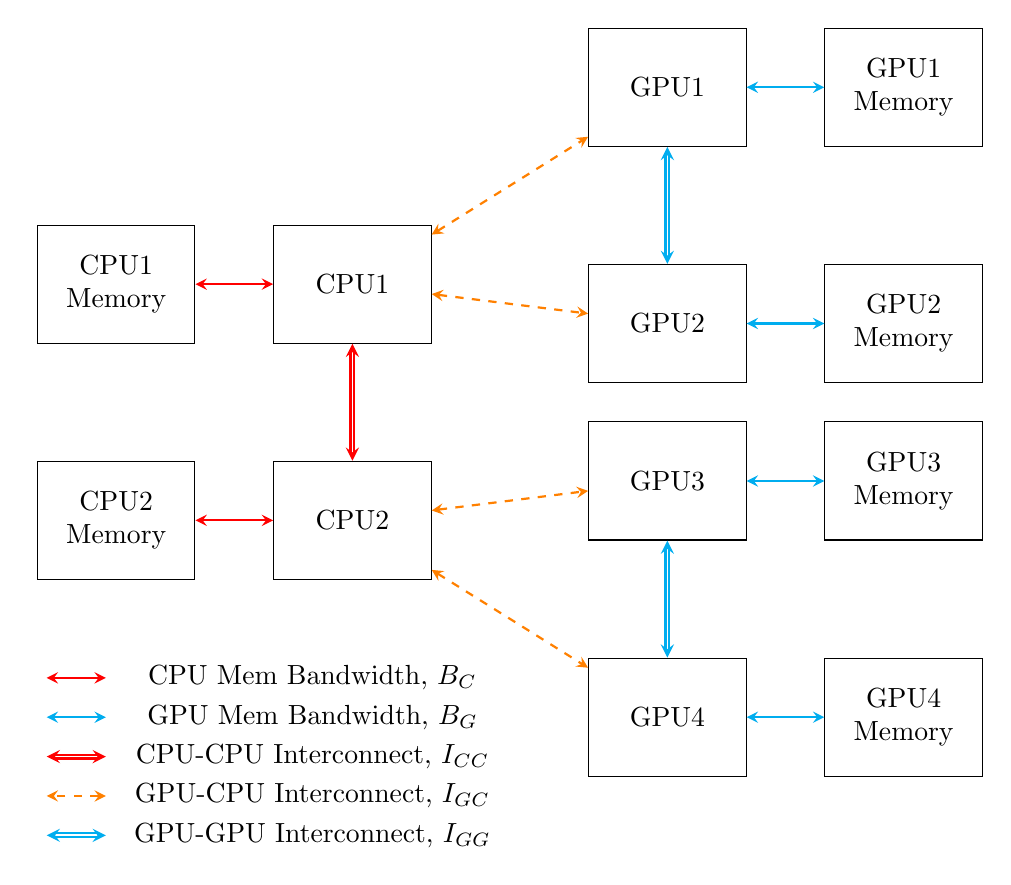
\begin{tikzpicture}
			
			\node[rectangle,
			draw = black,
			text = black,
			anchor = west,
			fill = white,
			align=center,
			minimum width = 2cm, 
			minimum height = 1.5cm] (cpu1) at (0cm,1.5cm) {CPU1};
			
			\node[rectangle,
			draw = black,
			text = black,
			anchor = west,
			fill = white,
			align=center,
			minimum width = 2cm, 
			minimum height = 1.5cm] (cpu2) at (0cm,-1.5cm) {CPU2};
			
			\node[rectangle,
			draw = black,
			text = black,
			anchor = west,
			fill = white,
			align=center,
			minimum width = 2cm, 
			minimum height = 1.5cm] (cpum1) at (-3cm,1.5cm) {CPU1 \\ Memory};
			
			\node[rectangle,
			draw = black,
			text = black,
			anchor = west,
			fill = white,
			align=center,
			minimum width = 2cm, 
			minimum height = 1.5cm] (cpum2) at (-3cm,-1.5cm) {CPU2 \\ Memory};
			
			
			\node[rectangle,
			draw = black,
			text = black,
			anchor = west,
			fill = white,
			align=center,
			minimum width = 2cm, 
			minimum height = 1.5cm] (gpu1) at (4cm,4cm) {GPU1};
			
			\node[rectangle,
			draw = black,
			text = black,
			anchor = west,
			fill = white,
			align=center,
			minimum width = 2cm, 
			minimum height = 1.5cm] (gpu2) at (4cm,1cm) {GPU2};
			
			\node[rectangle,
			draw = black,
			text = black,
			anchor = west,
			fill = white,
			align=center,
			minimum width = 2cm, 
			minimum height = 1.5cm] (gpu3) at (4cm,-1cm) {GPU3};
			
			\node[rectangle,
			draw = black,
			text = black,
			anchor = west,
			fill = white,
			align=center,
			minimum width = 2cm, 
			minimum height = 1.5cm] (gpu4) at (4cm,-4cm) {GPU4};
			
			\node[rectangle,
			draw = black,
			text = black,
			anchor = west,
			fill = white,
			align=center,
			minimum width = 2cm, 
			minimum height = 1.5cm] (gpum1) at (7cm,4cm) {GPU1 \\ Memory};
			
			\node[rectangle,
			draw = black,
			text = black,
			anchor = west,
			fill = white,
			align=center,
			minimum width = 2cm, 
			minimum height = 1.5cm] (gpum2) at (7cm,1cm) {GPU2 \\ Memory};
			
			\node[rectangle,
			draw = black,
			text = black,
			anchor = west,
			fill = white,
			align=center,
			minimum width = 2cm, 
			minimum height = 1.5cm] (gpum3) at (7cm,-1cm) {GPU3 \\ Memory};
			
			\node[rectangle,
			draw = black,
			text = black,
			anchor = west,
			fill = white,
			align=center,
			minimum width = 2cm, 
			minimum height = 1.5cm] (gpum4) at (7cm,-4cm) {GPU4 \\ Memory};
			
			
			\draw[red,  thick, stealth-stealth] (cpum1) to (cpu1);
			\draw[red,  thick, stealth-stealth] (cpum2) to (cpu2);
			\draw[red, double,  thick, stealth-stealth] (cpu1) to (cpu2);
			
			
			\draw[orange, dashed,  thick, stealth-stealth] (cpu1) to (gpu1);
			\draw[orange, dashed,  thick, stealth-stealth] (cpu1) to (gpu2);
			\draw[orange, dashed,  thick, stealth-stealth] (cpu2) to (gpu3);
			\draw[orange, dashed,  thick, stealth-stealth] (cpu2) to (gpu4);
			
			\draw[cyan,  thick, stealth-stealth] (gpum1) to (gpu1);
			\draw[cyan,  thick, stealth-stealth] (gpum2) to (gpu2);
			\draw[cyan,  thick, stealth-stealth] (gpum3) to (gpu3);
			\draw[cyan,  thick, stealth-stealth] (gpum4) to (gpu4);
			
			\draw[cyan, double,  thick, stealth-stealth] (gpu1) to (gpu2);
			\draw[cyan, double,  thick, stealth-stealth] (gpu3) to (gpu4);
			
			
			\node(al) at (-2cm, -3.5cm) {};
			\node (ar) at (-3cm, -3.5cm) {};
			\node[align=left] () at (0.5cm, -3.5cm) {CPU Mem Bandwidth, $B_{C}$};
			\draw[red,  thick, stealth-stealth] (al) to (ar);
			
			\node(al) at (-2cm, -4cm) {};
			\node (ar) at (-3cm, -4cm) {};
			\node[align=left] () at (0.5cm, -4cm) {GPU Mem Bandwidth, $B_{G}$};
			\draw[cyan,  thick, stealth-stealth] (al) to (ar);
			
			\node (bl) at (-2cm, -4.5cm) {};
			\node (br) at (-3cm, -4.5cm) {};
			\node[align=left] () at (0.5cm, -4.5cm) { CPU-CPU Interconnect, $I_{CC}$};
			\draw[red, double,  thick, stealth-stealth] (bl) to (br);
			
			\node (cl) at (-2cm, -5cm) {};
			\node (cr) at (-3cm, -5cm) {};
			\node[align=left] () at (0.5cm, -5cm) { GPU-CPU Interconnect, $I_{GC}$};
			\draw[orange, dashed,  thick, stealth-stealth] (cl) to (cr);
			
			\node (dl) at (-2cm, -5.5cm) {};
			\node (dr) at (-3cm, -5.5cm) {};
			\node[align=left] () at (0.5cm, -5.5cm) { GPU-GPU Interconnect, $I_{GG}$};
			\draw[cyan, double,  thick, stealth-stealth] (dl) to (dr);
			
			
		\end{tikzpicture}
	\end{center}
\end{figure}

\subsection{Datapoints of Supercomputers}


In this section we introduce a table which lists all important data points for Piz Daint, Summit and Alps. We have choosen Piz Daint because we have the possibility to test the Code on its systems, Eiger because we can also access its systems and it will give us a good reference values, due to non hybrid architecture, meaning the nodes to not have GPU. Finally we analyse its performance on Summit, as its at the time of writing this thesis, one of the most capable supercomputers in the world.

\small
\begin{figure}[H]
	\begin{center}
		\resizebox{\textwidth}{!}{%
		\begin{tabular}{|@{} c | c | c | c | }
			Constant & Piz Daint \cite{piz_daint} & Summit\cite{summit} & Alps (Eiger) \\ 
			\hline
			\# Nodes & 5704 & 4608 & 1024\\
			\# CPUs & 1 & 2 & 2\\
			CPU Model & Intel E5-2690 v3 \cite{E5-2690} & IBM POWER9 & AMD EPYC 7742\cite{AMDEPYC} \\
			CPU Mem. & 64 GB & 256 GB & ?? \\   
			$B_C$  & 68 GB/s & 170 GB/s & 204.8 GB/s x 2	\\
			$I_{CC}$ & - & 64 GB/s & ?? \\
			Base $GHZ_C$ & 2.9 GHZ & 4 GHZ & 2.25 GHZ\\
			Max $GHZ_C$ & 3.8 GHZ & 4 GHZ & 3.4 GHZ\\
			\# Cores & 12 & 22 & 64 \\
			Architexture & Haswell & & AMD Infinity Architecture \\
			Max AVX & AVX2 & ? & AVX2 \\ 
			\# GPUs & 1 & 6 & 0 \\
			GPU Model & NVIDIA P100 \cite{TESLAP100} & NVIDIA V100s \cite{NVIDIAV100} & - \\
			GPU Mem. Cap. & 16 GB & 16 GB $\times$ 6 & -\\
			$B_G$ & 732 GB/s & 900 GB/s $\times$ 6 & -\\
			$I_{GC}$ & 32 GB/s & 50 GB/s $\times$ 6 & -\\
			$I_{GG}$ & - & 50 GB/s & -\\
			GPU Tflops & 9,3 & 16.5 &\\
			\# CUDA Cores & 3584 & 5120 & \\
		\end{tabular}}	
	\end{center}
	\caption{Datapoints of Supercomputers}
	\label{fig:datapoints}
\end{figure}


\subsection{Model parameters}

\begin{comment}
If we investigate the operations which are needed for the binary cut algorithm, we notice that the actual operations completed inside the loop, are only very few. When comparing the CPU implementation with GPU one, we need to not only consider benefits from increased parallelism in GPU hardware, which will lead to a higher tflops, but also possible speed-ups reached by higher bandwidths in GPU memory than CPU memory. On the other hand we need to mitigate the very low bandwidths between the GPU and CPU, which cannot be avoided altogether, as the data needs to be sent from the CPU to GPU before we can process it on the graphics processor.
\end{comment}

In order to estimate the runtime of the algorithms we denote the number of particles as $N$. Furthermore we assume a precision $p$ of 32, which is general standard for both integers and floats, furthermore its a sensible assumption for astrophysical simulations. We only look at at the positional data of the particles for the runtime analysis since its the only relevant data to be considered to find a cut. The total storage of all particles is $32 \times 3 \times N bits = 4 \times 3 \times N Bytes = 12 \times N Bytes$. Furthermore we assume $d = 1024$ and $N=10^9$.


\subsection{Roofline Performance Model}

We test the our hypothesis, that ORB is, for the most part, memory bandwidth bound using the roofline model. In the roofline model, we compare the operational density, which is measured in FLOPS / per byte against the number of flops per minute. 

For modern hardware, its fairly uncommon to release a peak flops value. Since 2008 Intel has introduced AVX (Advanced Vector Extensions), benchmarks performance largely depend upon the compiled assembly instructions, where the specific instructions vary a lot between implementation details. SIMD instructions can only be used when there is a contiguous memory access. Thus the peformance of the code depends on chosen memory layout as well as iteration method. Due to the lack of peak flop estimations, we build our own model to estimate the flops of the major parts of ORB. 

AVX enables the processing of several floating point precision (32 bit) numbers simultaneously. AVX2, which is present in most modern hardware, enable the processing of 8 floating point instructions and its instructions have a CPI (cycles per instructions) of two on most chip architectures, where naturally a higher CPI correlates with an increased performance.

We define in equation \ref{eq:avx}, a function to estimate the number of gigaflops for a given hardware. We define GHZ as the gigahertz which can be reached by the CPU, meanwhile $NF$ is the number of floats which can be processed simultaneously using AVX. $CPI$ is as mentioned the cycles per instructions for the AVX instruction set. Finally we have $np$ which is the number of processors and  we assume a perfect parallelization, meaning 100\% of the code can be parallelized.

\begin{center}
	\begin{equation}
		gflops = GHZ * NF * CPI * np
	\end{equation}
\label{eq:avx}
\end{center}

In terms of arithmetic intensity, we take a look at the code for counting of particles left of a specified cut plane. We ignore other parts of the code for now, as optimizing this part is one of the main targets for the thesis. The part where we count the number of particles which are to the left of a cut position, essentially comes down to this loop:

\begin{figure}
	\begin{lstlisting}[language=c++]
		for(auto p= startPtr; p<endPtr; ++p) nLeft += *p < cut;
	\end{lstlisting}
\caption{Counting the particles left of a cut plane}
\end{figure}


Where $p$ is a C-style array which stores the particles position and $nLeft$ gives the number of particles which are left of the $cut$. In terms of arithmetic intensity, we have the following operations:

\Q{Add glossary for terms like arithemtic intensity?}

\begin{enumerate}
	\item Compare particle to cut
	\item Add result to $nLeft$
	\item Increment pointer $p$
	\item Compare pointer $p$ with $endPtr$
\end{enumerate}

Which results in a total of 4 operations. Since a single float is stored using 4 bytes, we receive 1.0 operations per byte. Note that AVX or any SIMD instructions do not influence the arithmetic intensity, as the number of floating point operations per byte remains the same. We simply perform a set of operations concurrently. What is however influenced by AVX, is the maximum number of GFLOPS which can be processed by the hardware. If we were to ignore AVX, the algorithm would clearly not be bound by memory, as its performance would lack behind the memory bandwidth. For this reason it is so important to consider AVX.

Since we have peak flops benchmarks available for all the NVIDIA P100 and V100s we do not need to make any estimations about the GPU flops. Estimating the arithmetic intensity for the GPU is a lot more complicated as it depends a lot on the specific implementation details. For now we will just assume the same arithmetic intensity as we have had for the CPU.

\begin{figure}[H]
	\begin{center}
		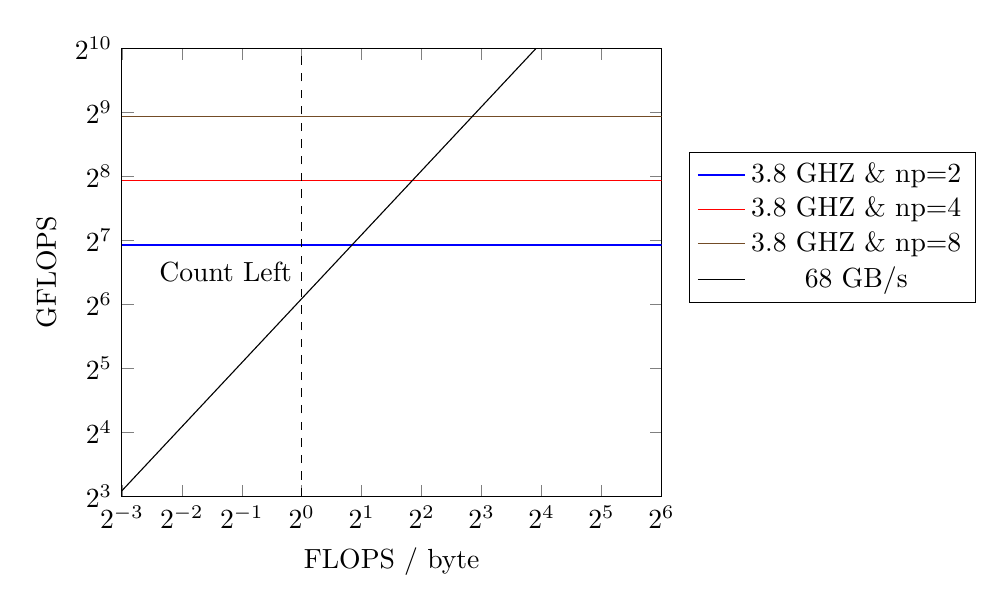
\begin{tikzpicture}
				\begin{axis}[
					xmode=log,
					ymode=log,
					log basis x={2},
					log basis y={2},
					xlabel={FLOPS / byte},
					ylabel={GFLOPS},
					%x filter/.code=\pgfmathparse{#1 + 6.90775527898214},
					xmin = 0.125, xmax = 64, ymin= 8, ymax=1024,
					legend style={at={(1.05,0.6)},anchor=west}]
			
					\addplot+[name path = A, domain = 0.125:64, mark=none] {
						3.8 * 8 * 2 * 2
					};	
					
					\addlegendentryexpanded{3.8 GHZ \& np=2};
					
					\addplot+[name path = A, domain = 0.125:64, mark=none] {
						3.8 * 8 * 2 * 4
					};	
					
					\addlegendentryexpanded{3.8 GHZ \& np=4};
					
					\addplot+[name path = A, domain = 0.125:64, mark=none] {
						3.8 * 8 * 2 * 8
					};	
					
					\addlegendentryexpanded{3.8 GHZ \& np=8};
					
					\addplot+[name path = A, domain = 0.125:64, mark=none] {
						68 * \x
					};	
					
					\addlegendentryexpanded{68 GB/s};
					
		
					\draw[dashed] (axis cs:1,8) -- node[left]{Count Left} (axis cs:1,1024);
					
				\end{axis}
			\end{tikzpicture}
	\caption{Roofline Model for Piz Daint CPU}
	\label{fig:roofdaint}
	\end{center}
\end{figure}


\begin{figure}[H]
	\begin{center}
		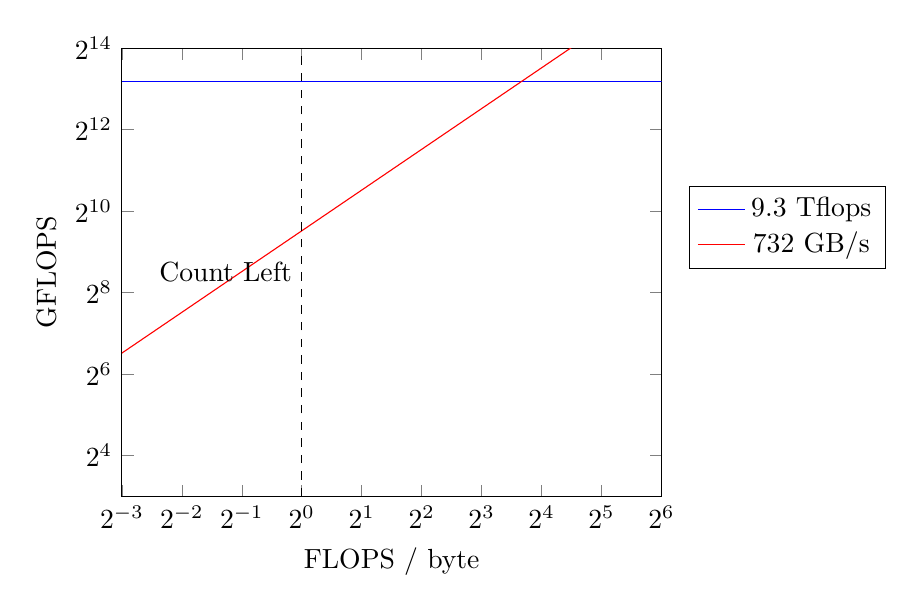
\begin{tikzpicture}
			\begin{axis}[
				xmode=log,
				ymode=log,
				log basis x={2},
				log basis y={2},
				xlabel={FLOPS / byte},
				ylabel={GFLOPS},
				%x filter/.code=\pgfmathparse{#1 + 6.90775527898214},
				xmin = 0.125, xmax = 64, ymin= 8, ymax=16384,
				legend style={at={(1.05,0.6)},anchor=west}]
				
				\addplot+[name path = A, domain = 0.125:64, mark=none] {
					9300
				};	
				
				\addlegendentryexpanded{9.3 Tflops};
				
				\addplot+[name path = A, domain = 0.125:64, mark=none] {
					732 * \x
				};	
				
				\addlegendentryexpanded{732 GB/s};
				
				
				\draw[dashed] (axis cs:1,8) -- node[left]{Count Left} (axis cs:1,16384);
				
			\end{axis}
		\end{tikzpicture}
		\caption{Roofline Model for Piz Daint GPU}
		\label{fig:roofdaintGPU}
	\end{center}
\end{figure}

As it can be seen in figure \ref{fig:roofdaint} and \ref{fig:roofdaintGPU} both the GPU and CPU version running on Piz Daint are memory bound, but due to its much higher memory bandwidth limit, a GPU version should be favored. 

\begin{figure}[H]
	\begin{center}
		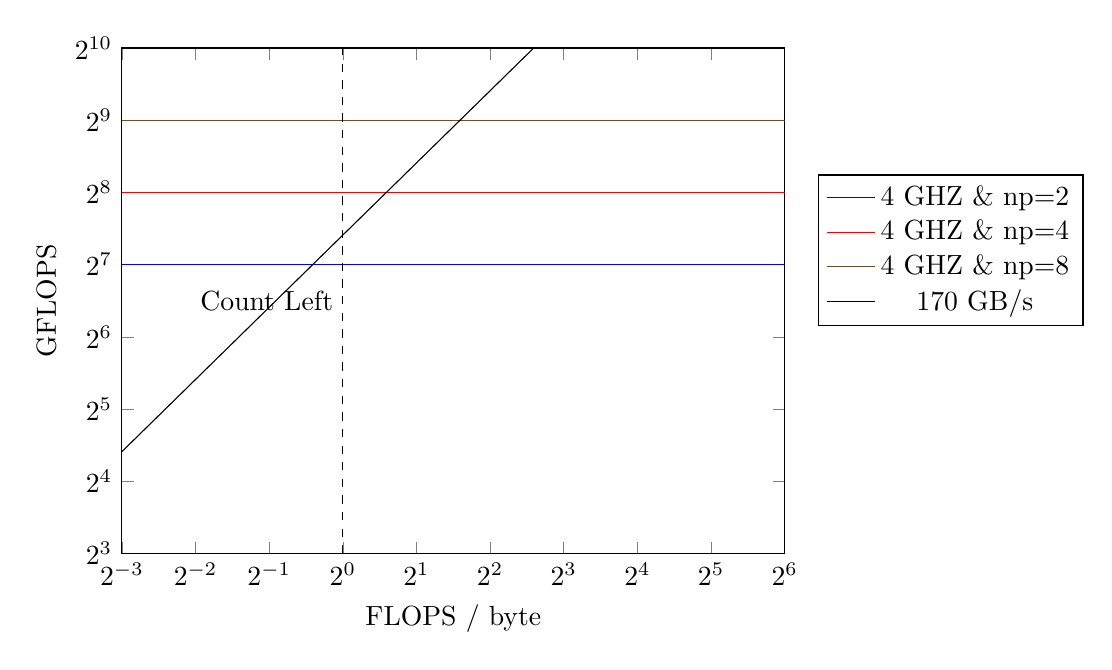
\begin{tikzpicture}
			\begin{axis}[
				xmode=log,
				ymode=log,
				log basis x={2},
				log basis y={2},
				height=8cm,width=10cm, 
				xlabel={FLOPS / byte},
				ylabel={GFLOPS},
				%x filter/.code=\pgfmathparse{#1 + 6.90775527898214},
				xmin = 0.125, xmax = 64, ymin= 8, ymax=1024,
				legend style={at={(1.05,0.6)},anchor=west}]
				
				
				\addplot+[name path = A, domain = 0.125:64, mark=none] {
					4 * 8 * 2 * 2
				};	
				
				\addlegendentryexpanded{4 GHZ \& np=2};
				
				\addplot+[name path = A, domain = 0.125:64, mark=none] {
					4 * 8 * 2 * 4
				};	
				
				
				\addlegendentryexpanded{4 GHZ \& np=4};
				
				\addplot+[name path = A, domain = 0.125:64, mark=none] {
					4 * 8 * 2 * 8
				};	
				
				
				\addlegendentryexpanded{4 GHZ \& np=8};
				
				\addplot+[name path = A, domain = 0.125:64, mark=none] {
					170 * \x
				};	
				
				\addlegendentryexpanded{170 GB/s};
				
				
				\draw[dashed] (axis cs:1,8) -- node[left]{Count Left} (axis cs:1,1024);
			
				
			\end{axis}
		\end{tikzpicture}
	\end{center}
	\caption{Roofline Model for Summit}
	\label{fig:roofsummit}
\end{figure}


\begin{figure}[H]
	\begin{center}
		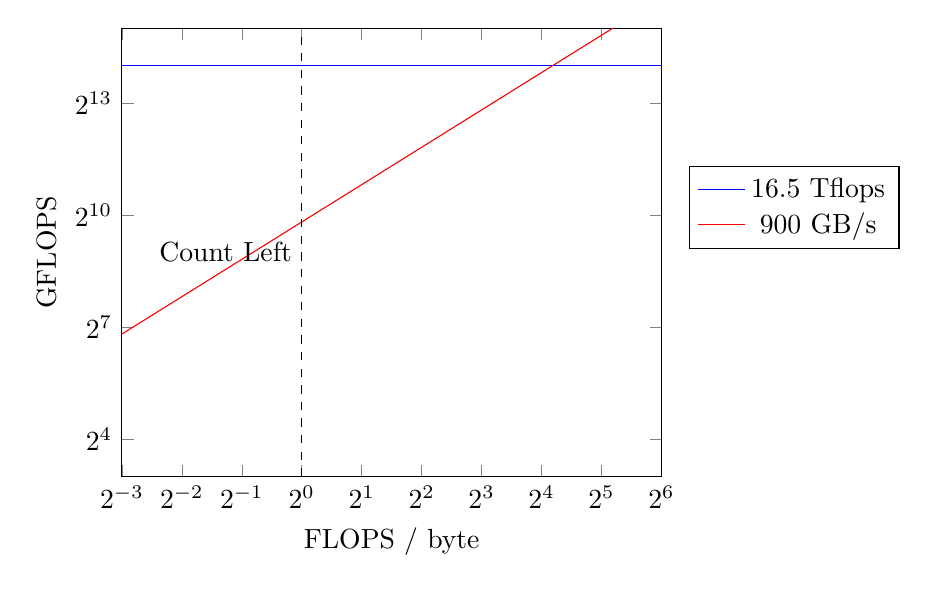
\begin{tikzpicture}
			\begin{axis}[
				xmode=log,
				ymode=log,
				log basis x={2},
				log basis y={2},
				xlabel={FLOPS / byte},
				ylabel={GFLOPS},
				%x filter/.code=\pgfmathparse{#1 + 6.90775527898214},
				xmin = 0.125, xmax = 64, ymin= 8, ymax=32768,
				legend style={at={(1.05,0.6)},anchor=west}]
				
				\addplot+[name path = A, domain = 0.125:64, mark=none] {
					16500
				};	
				
				\addlegendentryexpanded{16.5 Tflops};
				
				\addplot+[name path = A, domain = 0.125:64, mark=none] {
					900 * \x
				};	
				
				\addlegendentryexpanded{900 GB/s};
				
				
				\draw[dashed] (axis cs:1,8) -- node[left]{Count Left} (axis cs:1,32768);
				
			\end{axis}
		\end{tikzpicture}
		\caption{Roofline Model for Summit GPU}
		\label{fig:roofsummitGPU}
	\end{center}
\end{figure}

As visible in figure \ref{fig:roofsummit} and \ref{fig:roofsummitPGU} the same applies to Summit. Its notable how the memory bandwidth only becomes the limiting factor when assuming a parallelization with 4 processors.

\begin{figure}
	[H]
	\begin{center}
		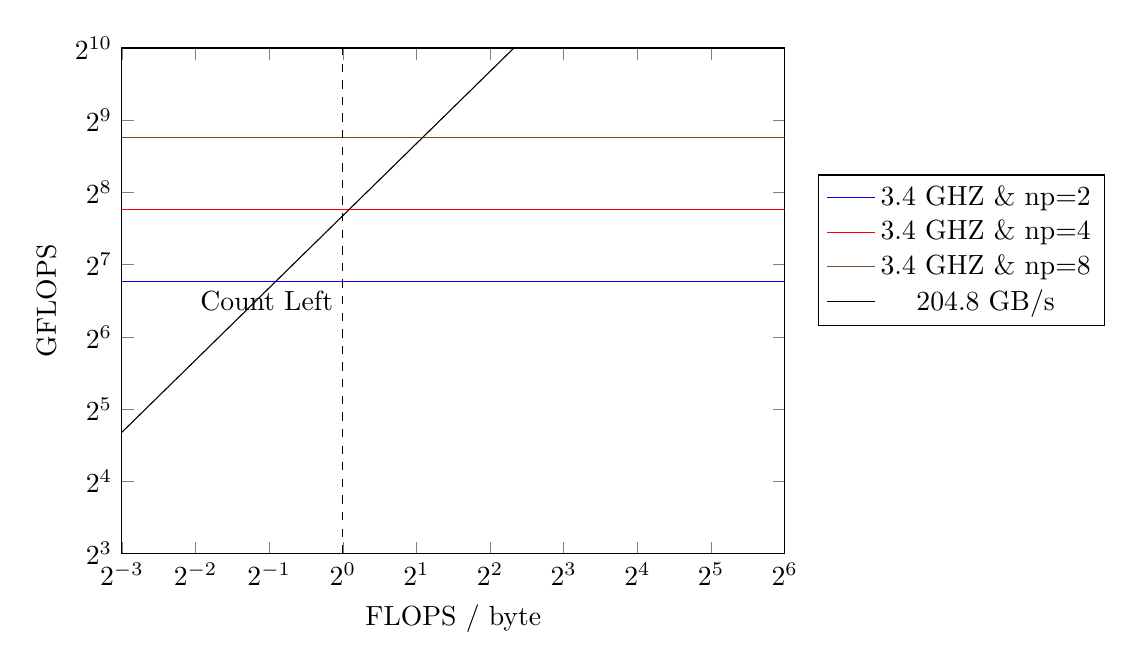
\begin{tikzpicture}
			\begin{axis}[
				xmode=log,
				ymode=log,
				log basis x={2},
				log basis y={2},
				height=8cm,width=10cm, 
				xlabel={FLOPS / byte},
				ylabel={GFLOPS},
				%x filter/.code=\pgfmathparse{#1 + 6.90775527898214},
				xmin = 0.125, xmax = 64, ymin= 8, ymax=1024,
				legend style={at={(1.05,0.6)},anchor=west}]
				
				
				\addplot+[name path = A, domain = 0.125:64, mark=none] {
					3.4 * 8 * 2 * 2
				};	
				
				\addlegendentryexpanded{3.4 GHZ \& np=2};
				
				\addplot+[name path = A, domain = 0.125:64, mark=none] {
					3.4 * 8 * 2 * 4
				};	
				
				\addlegendentryexpanded{3.4 GHZ \& np=4};
				
				\addplot+[name path = A, domain = 0.125:64, mark=none] {
					3.4 * 8 * 2 * 8
				};	
				
				\addlegendentryexpanded{3.4 GHZ \& np=8};
				
				\addplot+[name path = A, domain = 0.125:64, mark=none] {
					204.8 * \x
				};	
				
				\addlegendentryexpanded{204.8 GB/s};
				
				\draw[dashed] (axis cs:1,8) -- node[left]{Count Left} (axis cs:1,1024);
				
				
			\end{axis}
		\end{tikzpicture}
	\end{center}
	\caption{Roofline Model for Alps}
	\label{fig:roofalps}
\end{figure}

Finally alps, which has the highest memory bandwidth compared to its flops, also becomes limited by the bandwidth after using more than four processors.
We consider a minimal C++ code to make measurements which can prove the theoretical model. We use the -S flag along with the g++ compiler to generate assembly code from the c++ source code and make sure that AVX commands are enabled. For testing purposes all entries in the array are set to random values between 0 and 1, and cut is set to 0.5.

In a first test, we do not enable AVX, but turn on $O3$. The generated assembly code looks as follows:

\begin{figure}[H]
	\begin{lstlisting}
.L18:
	movups	(%rax), %xmm0
	addq	$16, %rax
	cmpltps	%xmm2, %xmm0
	psubd	%xmm0, %xmm1
	cmpq	%rdx, %rax
	jne	.L18

	\end{lstlisting}
\caption{Reduction Assembler Code without AVX}
\label{fig:assembler}
\end{figure}
$psubd$ is a packaged instruction, meaning it already uses some form of SIMD instructions. The command is used in the MME and later the SSE2 instruction set. Since we can observe that the $xmm$ registers are used, we know its a SSE2 instruction. 

If we additionally set the compile flag -march=native we end up with the following code:

\begin{figure}[H]
\begin{lstlisting}
.L19:
	vmovups	(%rax), %ymm3
	addq	$32, %rax
	vcmpltps	%ymm2, %ymm3, %ymm0
	vpsubd	%ymm0, %ymm1, %ymm1
	cmpq	%rdx, %rax
	jne	.L19	

\end{lstlisting}
\caption{Reduction Assembler Code with AVX2}
\label{fig:assembler-avx}
\end{figure}

We can identify $vmovups$, $vcomplpts$ and $vpsubd$ which are all AVX commands. Since they are using the ymm instead of the xmm registers, we know these are AVX2 and not AVX commands. For the chip architecture we have tested this on, AVX2 is the most optimal SIMD instruction set.

\TODO{Fix, Redo this part}
The following test results were achieved from a Intel(R) Core(TM) i9-10885H CPU @ 2.40GHz
processor. We perform the conditional reduction on  $2^{27}$ particles. The reduction takes 244420 microseconds. This means we have a throughput of $2^{27} / 10^{12} * 10^6 / 24420 = 0.00549 tflops$. This of course does not lie anywhere near the theoretical maximum, which even for a single processor ($np = 1$) is $2.4 * 8 * 2 * 1 / 1000 = 0.0384 tflops.$. This is a strong indication, that already with a single processor solutions, we are in the realm of bandwidth limited algorithms. This effect of course, would become even stronger when including parallelism.

But regardless if the app is actually memory bound or not, fact is that the GPU outperforms the CPU by a factor of 10-20 $\times$, thus even if it were bound by the chip architecture, there is still an improvement to be expected when porting the code to the GPU. 

\subsection{Models for different approaches}

When building the models, we assume that ORB is memory bound. Meaning that the limiting factor is not the flops of the chip, but rather the memory bandwidth. We will construct and explore models for three different approaches. In the first naive implementation, we simply send an array of particles to the GPU, where the counting is then performed. In a more advanced variant, we consider sending the particles from the CPU to GPU only once and perform the partitioning on the GPU as well.  
 
\subsubsection{GPU Counting}

Each time we split all leaf cells into two child cells, we end up with twice the amount of cells. Considering we want to end up with $d$ leaf cells in the end, we need to perform the cut algorithm $log(d)$ times, which corresponds to the height of the tree. Each time we perform the cut algorithm, we test a maximum of $p$ different cut guesses. As we traverse the tree the number of cells increases, but at the same time the number of particles which need to counted decrease by the same factor. Thus the amount of cells which are to be iterated cancels out and we end up with the size of all particles $s$ divide by the memory bandwidth $B_C$.  
 
\begin{center}
	\begin{equation}
			log(d) \times \left ( p \times \frac{ s }{B_{C}} \right ) = t
			\label{eq:cpu}
	\end{equation}
\end{center}

\vspace{5mm}


The Equation \ref{eq:gpu} for the GPU is similar, the only difference being that we use the GPU memory bandwidth $B_{GPU}$ instead of the CPU bandwidth. Furthermore we have to consider the time it takes to send the data from the CPU to the GPU. This adds the terms size divided by CPU to GPU memory bandwidth denoted as $I_{GC}$. Finally we also need to load the data from the CPU memory to the CPU before we are able to send it. 

\begin{center}
	\begin{equation}
			log(d) \times \left ( p \times \frac{s}{B_{G}} + \frac{s}{I_{GC}}  + \frac{s}{B_{C}} \right ) = t
		\label{eq:gpu}
	\end{equation}
\end{center}

\vspace{5mm}


\subsubsection{GPU Counting and Partitioning}\label{gpu-tree-building}

We can also consider performing the partitioning on the GPU, this means that there is no need to send data from the CPU to GPU each time we want to find a cut, allowing us to reduce the costly overheads. This means that we are able to move the considering the CPU GPU bandwidths and the initial loading data out of the bracket and reducing the runtime.

\begin{center}
	\begin{equation}
		log(d) \times \left ( p \times \frac{s}{B_{G}} \right ) + \frac{s}{I_{GC}} + \frac{s}{B_{C}} = t
		\label{eq:gputree}
	\end{equation}
\end{center}


\begin{comment}
\subsubsection{Batch loading}

Finally we can also try to mitigate the overheads introduced by CPU to GPU communication by sending small batches, such that the GPU can already start processing the data, before the data transfer was completed. Lets denote the number of batches by $b$. For the sake of simplicity we only make a single cut and thus can reuse Equation \ref{eq:cpu} for the CPU version. For the GPU we now omit the term for memory access from the GPU. Because we can already start processing data in parallel when the first batch arrived and $B_{G} > I_{GC}$ holds for every modern hardware. Thus the only overhead we still get is $\frac{s \div b}{B_{G}}$ for the very last batch, but as we can just increase b in relation to N, this becomes negligible. Note that this only counts for the very first iteration, thus the only difference we have is the constant of 31 and not 32. 

\begin{center}
	\begin{equation}
		(d-1) \times p \times \frac{s}{B_{G}} + 2 \times \frac{s}{I_{GC}} = t
		\label{eq:gpubatch}
	\end{equation}
\end{center}

Due to possible overhead and no real improvement over the naive GPU version, we will omit the analysis using this method.

\subsubsection{Data compression}

Since for most computer the Interconnect bandwidth is greatly smaller than the Memory bandwidth, we could potentially also think about compressing the particle data. This would increase computational costs, but would allow us to store a higher amount of particles and reduce the cost which comes from loading the particles from memory as well as sending the data over the Interconnect.

\begin{itemize}
	\item Why do we even use floats in the first place? wouldn't integers suit better since precision is uniformly equal?
	\item Reduce transferred number of bits, sacrifice precision?
\end{itemize}

\TODO{Add plots?}

\end{comment}
\newcommand\s{12}

\newcommand\p{32}

%\newcommand\d{1024}

\normalfont
\subsection{Piz Daint} 

Let us plugin the values from figure \ref{fig:datapoints} into the corresponding formulas \ref{eq:cpu}, \ref{eq:gpu} and \ref{eq:gputree} for piz daint.

\subsubsection{Naive implementation}
The naive implementation yields the following speeds for the naive CPU  implementation:

\pgfmathsetmacro\cpuPiz{ln(1024) / ln(2) * (\p * \s / 68)}

\begin{center}
	\begin{equation}
		log(1024) \times \left ( \p \times \frac{ \s GB }{68 GB/s} \right )  = \cpuPiz s
	\end{equation}
\end{center}


And the corresponding GPU implementation:
\pgfmathsetmacro\gpuPizN{ ln(1024) / ln(2) * (\p * \s / 732 + \s / 32 + \s / 68)}
\begin{center}
	\begin{equation}
		log(1024) \times \left ( 32 \times \frac{12 GB}{732 GB/s} + \frac{12 GB}{32 GB/s}  + \frac{12 GB}{68 GB/s} \right )=  \gpuPizN s
	\end{equation}
\end{center}

This yields in a speed-up of:
\pgfmathsetmacro\speedup{\cpuPiz / \gpuPizN}
\begin{center}
	\begin{equation}
		\frac{\cpuPiz}{\gpuPizN} = \speedup \times
	\end{equation}
\end{center}


\subsubsection{GPU Tree Building}

And the corresponding GPU implementation:
\pgfmathsetmacro\gpuPizT{ ln(1024)/ln(2) * (\p * \s / 732)  + \s / 32 + \s / 68}
And the corresponding GPU implementation:
\begin{center}
	\begin{equation}
		log(1024) \times \left ( \p \times \frac{\s GB}{732 GB/s} \right ) + \times \frac{\s GB}{32 GB/s}  + \frac{\s GB}{68 GB/s} = \gpuPizT s
	\end{equation}
\end{center}

This yields in a speed-up of:
\pgfmathsetmacro\speedup{\cpuPiz / \gpuPizT}
\begin{center}
	\begin{equation}
		\frac{\cpuPiz}{\gpuPizT} = \speedup \times
	\end{equation}
\end{center}

\vspace{5mm}

\pgfmathsetmacro\cpuSummit{ln(1024) / ln(2) * (\p * \s / (170 * 2)}
\pgfmathsetmacro\gpuSummitN{ln(1024) / ln(2) * (
	(\p * \s / (900 * 6) + 
	\s / (50 * 6) + \s /(170 * 2)
	)}
\pgfmathsetmacro\gpuSummitT{ln(1024) / ln(2) * 
	(\p * \s / (900 * 6))
	+  \s / (50 * 6) + \s /(170 * 2)}
\pgfmathsetmacro\cpuEiger{ln(1024) / ln(2) * (\p * \s / (204.8 * 2)}
 
The computations for Eiger and Summit can performed in the same way as we have shown for Piz Daint. For Eiger we cannot make any assumption for a GPU version as its CPU only system.

\begin{comment}

\subsection{Summit}

Let us plugin the values from Figure \ref{fig:datapoints} into the corresponding formulas \ref{eq:cpu}, \ref{eq:gpu}, \ref{eq:cputree} and \ref{eq:gputree}.

\subsubsection{Naive implementation}
The naive implementation yields the following speeds for the naive CPU  implementation:


\begin{center}
	\begin{equation}
		log(1024) \times \left ( \p \times \frac{ \s GB }{170 GB/s \times 2} \right ) = \cpuSummit s
	\end{equation}
\end{center}

And the corresponding GPU implementation:

\begin{center}
	\begin{equation}
		log(1024) \times \left ( \p \times \frac{\s GB}{900 GB/s \times 6} + \frac{\s GB}{50 GB/s \times 6}  + \frac{\s GB}{170 GB/s \ \times 2} \right )= \gpuSummitN s
	\end{equation}
\end{center}

This yields in a speed-up of:
\pgfmathsetmacro\speedup{\cpuSummit / \gpuSummitN}
\begin{center}
	\begin{equation}
		\frac{\cpuSummit s}{\gpuSummitN s} = \speedup \times 
	\end{equation}
\end{center}


\subsubsection{GPU Tree Building}

And the corresponding GPU implementation:

\begin{center}
	\begin{equation}
		log(1024) \times \left ( \p \times \frac{\s GB}{900 GB/s \times 6} \right ) + \frac{\s GB}{50 GB/s \times 2}  + \frac{\s GB}{170 GB/s \times 2} = \gpuSummitT s
	\end{equation}
\end{center}

This yields in a speed-up of:
\pgfmathsetmacro\speedup{\cpuSummit / \gpuSummitT}
\begin{center}
	\begin{equation}
		\frac{\cpuSummit s}{\gpuSummitT s} = \speedup \times
	\end{equation}
\end{center}


\vspace{5mm}


\subsection{Eiger}

\pgfmathsetmacro\cpuEiger{ln(1024) / ln(2) * (\p * \s / (204.8 * 2)}

\begin{center}
	\begin{equation}
		\log(1024) \times \p \times \frac{ \s GB }{204.8 GB/s \times 2} = \cpuEiger s
	\end{equation}
\end{center}

\end{comment}

\subsection{Conclusion}

We conclude that the GPU version with GPU Tree building enabled yields the best speedup and also performs a lot better than the CPU version. Furthermore we can observe that the speedup is bounded by $\frac{B_{GPU}}{B_{CPU}}$/, because both the CPU and GPU implemented version are ultimately limited by the bandwidth.

\begin{figure}[H]
	\begin{center}
		\begin{tikzpicture}
			
			\begin{axis} [ybar,height=10cm,width=13cm, 
				bar width=0.8cm,
				enlargelimits=0.2,
				symbolic x coords={Piz, Summit, Eiger},
				legend columns=1,
				legend entries={CPU, Hybrid Naive, Hybrid Tree},
				ylabel={Runtime (s) },
				x tick label style={rotate=45,anchor=east}, 
				xtick=data]
				\addplot coordinates {
					(Piz,\cpuPiz ) 
					(Summit,\cpuSummit) 
					(Eiger,\cpuEiger) 
				};
			
				\addplot coordinates {
					(Piz,\gpuPizN ) 
					(Summit,\gpuSummitN ) 
				};
			
				\addplot coordinates {
					(Piz,\gpuPizT ) 
					(Summit,\gpuSummitT  ) 
				};
			\end{axis}
			
		\end{tikzpicture}
	\end{center}

\caption{Execution times of different strategies}
\label{fig:exectimes}
\end{figure}




\begin{comment}
\begin{figure}
\begin{center}
\begin{tikzpicture}
\begin{axis}[xmin = -1, xmax = 13, ymin=-1, ymax=6]
\addplot[domain = 0:12,blue] {ln(1024) / ln(2) * 
(\p * x / (900 * 6))
+  x / (50 * 6) + x /(170 * 2)};
\addplot[domain = 0:12,blue] {ln(1024 * 16) / ln(2) * 
(\p * x / (900 * 6))
+  x / (50 * 6) + x /(170 * 2)};
\end{axis}
\end{tikzpicture}
\end{center}
\caption{??}
\label{fig:exectimes}
\end{figure}

\end{comment}

\newpage
\section{Implementation}

In this section we will describe the stand-alone implementation of the accelerated ORB algorithm. We will develop this somewhat separately from the PKDGrav codebase in order to have smaller and easily understandable codebase. We will however use mdl2 from PKDGrav, which is used to distribute the workload among the processors in the system. We aim to use this platform for extensive empirical testing of different strategies and evaluate weather our the proposed method indeed outperforms the CPU version. 

We will not describe every part of the code in detail, as this would exceed the scope of the thesis. However any performance critical details and all the important data-structures are described. Furthermore, we will pay special attention to the CUDA kernels and also memory management strategies, as they are of great importance.

A brief overview of the core elements:

\begin{itemize}
	\item \textbf{particles}: The particles array has ownership over all particle objects. It has the shape of a multidimensional array, where the first three axes are occupied by positional data and the rest can be filled with meta data.
	\item \textbf{Cell}: The cell class is a structure keeping track of the fundamental cell information. In essence it is the analogue to the concept of the $cell$ which we have already introduced in section \ref{section:orb}.
	\item \textbf{Services}: The services are a set of functions, which together form the building block of the ORB algorithm. This abstraction layer allows us to dynamically distribute and collect tasks from different processors. Each service builds on top of a PST class which is introduced by mdl2.
	
\end{itemize}

For this project we will use C++ 17 along with CUDA 11.3, OpenMPI 4.1.0 and Blitz++ 1.0.2 \cite{blitzcpp}. 

\subsection{MDL}

Briefly explain how mdl exactly works. 

\subsection{Particles}

To implement the particles array, we use C-style arrays interchangeably with blitz++ arrays. The blitz++ array is a wrapper class around C-style arrays, which helps with pointer management and can speed up the debugging process by keeping track of the array size and checking access indexes. Furthermore, we can easily create slices and make borrowed copies. 
Blitz++ allows us to easily access the C-style array with the command $array.data()$, enabling us to switch to C-style arrays, whenever its deemed necessarily. 

The particles array is essentially a 2D array where each row represents a single particle. Since the performance critical part, the binary cut algorithm, of ORB only iterates over a single axis, we can further enhance the performance by choosing a column major storage format. This ensures that memory accesses are happening over consecutive data, and cache misses are limited.

We have observed cases, where iterating over a blitz array does not enable AVX, even though in theory the storage order would allow so. However iterating over the underlying C-style array did enable AVX.

\subsection{Mapping cells to particles}

Since only the operative needs to keep track of the cells, we need a separate data-structure which defines the range of particles which are encompassed inside the volume of a cell, for each thread. We solve this problem with a 2D array, where we map from a cell ID to its start index in the particles array, as well as its end index. Of course, this array needs to be updated each time we perform a reshuffling.

\subsection{Cell}

The tree which is constructed by ORB consists of multiple cells and ultimately we need to find a suitable data-structure. The most obvious choice is a tree, which keeps track of its children using pointers. But as we have seen in section \ref{section:orb-example} the conditions for a nearly complete binary tree hold, allowing for a heap to be used as storage method for the tree. The heap A heap of course has constant $O(1)$ access times over $O(log(d))$ for the tree.


\begin{figure}[H]
	\begin{center}
		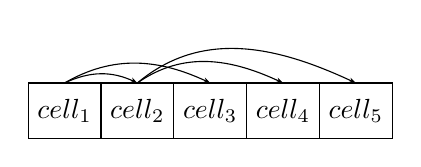
\begin{tikzpicture}[
			%  -{Stealth[length = 2.5pt]},
			start chain = going right,
			node distance = 0pt,
			MyStyle/.style={draw, minimum width=2em, minimum height=2em, 
				outer sep=0pt, on chain},
			]
			\node [MyStyle] (1) {$cell_1$};
			\node [MyStyle] (2) {$cell_2$};
			\node [MyStyle] (3) {$cell_3$};
			\node [MyStyle] (4) {$cell_4$};
			\node [MyStyle] (5) {$cell_5$};
			\begin{scope}[-{Stealth[length = 2.5pt]}]
				\draw (1.north) [out=25, in=155] to (2.north);
				\draw (1.north) [out=30, in=155] to (3.north);
				\draw (2.north) [out=35, in=155] to (4.north);
				\draw (2.north) [out=40, in=155] to (5.north);
			\end{scope}
		\end{tikzpicture}
		\qquad
		\begin{figure}
			\Tree[.cell_1 [.cell_2 [.cell_4 ] [.cell_5 ] ]
			[.cell_3 ]]
		\end{figure}
	\end{center}
	\caption{Tree as heap}
\end{figure}

When a heap array exceeds its allocated memory space, we need to reallocate memory, which can be very time intensive, especially for very large arrays. In our case however, its possible to set an upper boundary for the maximum number of cells. Another positive aspect of the heap is that the interface of mdl2 requires data to be sent in an array structure anyways, further decreasing performance loss and algorithmic complexity.


Since the last level of the tree, in cases when $d$ s not a power of two, is only partially filled with leaf nodes, we need to be careful when applying the algorithm. However we can derive all crucial metrics for a given tree, based on the basic heap conditions.

\subsubsection{Heap Conditions}
As with all heap data-structures we have the following conditions:

\begin{itemize}
	\item The root cell has index 1
	\item The left child of cell at index $i$ can be accessed at the index $i\times2$. 
	\item The left child of cell at index $i$ can be accessed at the index $i\times2 + 1$. 
\end{itemize}

\vspace{0.5cm}
Furthermore we can derive the following constraints given the number of leaf cells $d$:

\begin{itemize}
	\item We can compute the depth of the tree with: $\lceil log_2(d) \rceil$
	\item The number of leaf cells on the second last level is given by $2^{depth} - d$ 
	\item There are exactly $2 \times d - 2^{depth}$ items (which must all be leaf cells) on the last level. 
	\item The total number of cells are $2\times d - 1$.
\end{itemize}

\subsubsection{Class}
The cell class consists of the following variables:

\begin{itemize}
	\item $id$: The id is a unique identification of the cell instance.
	\item $nLeafCells$: this variable is equal to $d_{cell}$ and depicts the number of leaf cells which can be found when walking all possible child cells of this cell. 
	\item $lower$: The lower is 3D point coordinate which represents the lower boundary corner of the 3D volume $V_{cell}$ which is encompassed by this cells domain.
	\item $upper$: The represents the upper boundary corner of the volume.	
	\item $tmp$: The cell has room for additional data, which may be stored during executions of algorithms. 
\end{itemize}

\subsection{Operative}

Describe operative code here. Mention why we use for loop instead of recursive version. Inlcude code? -> quiet long

\subsection{Services}

As required by mdl, we make use of services, which are essentially a collection of functions which can be sent to any set of processors in the computing system. We abstract every performance critical part of the orb main runtime, which can parallelized and distributed among processors.

The services we have implemented and which are crucial for the CPU version are:

\begin{itemize}
	\item $init$ : Reads the particles and allocates memory on the CPU accordingly.
	\item $finallize$ : Frees all the memory and ensures a memory leak free execution.  
	\item $countLeft$ : Counts the number of particles left of a provided cut position for each of the cells.
	\item $count$ : Counts the total number particles inside the domain for each of the provided cells.
	\item $partition$ : Partitions the particles to preserve memory locality.
\end{itemize}

\subsubsection{Count Left}

The countLeftService takes as a input an array of cells and stores the counts in an output array. Each cell comes with a cut position and a cut axis, thus the service counts the number of particles to the left of this position in the given axis. 

As for every service, we have access to the input array with a pointer to its first element in memory called $in$ and correspondingly $out$ for the output array. We then iterate over the number of cells and access the cell structure given the cellPtrOffset as seen on line number two.
We then check weather the proper cut has already been found, if so we directly continue with the next cell (Line 4-6). We use the cellToRangeMap, which is stored as local data of the pst to retrieve the begin and end index of this cell in the particles array. (Line 7-8).
We then take a slice of the particles array and store a pointer to the data in $startPtr$ and correspondingly compute the end pointer as well. (10-14).
Finally we simple iterate over the particles and count up, as previously mentioned, this can enable AVX, given hardware support and the proper compile flags. Usually $-march=native$ along with $O3$ will enable AVX. 

\begin{lstlisting}[language=c++]
 for (int cellPtrOffset=0; cellPtrOffset<nCells; ++cellPtrOffset){
	auto cell = static_cast<Cell>(*(in + cellPtrOffset));
	
	if (cell.foundCut) {
		continue;
	}
	int beginInd = pst->lcl->cellToRangeMap(cell.id, 0);
	int endInd =  pst->lcl->cellToRangeMap(cell.id, 1);
	
	blitz::Array<float,1> particles =
		pst->lcl->particlesAxis(blitz::Range(beginInd, endInd));
	
	float * startPtr = particles.data();
	float * endPtr = startPtr + (endInd - beginInd);
	
	int nLeft = 0;
	float cut = cell.getCut();
	for(auto p= startPtr; p<endPtr; ++p)
	{
		nLeft += *p < cut;
	}
	
	out[cellPtrOffset] = nLeft;
}
\end{lstlisting}


\subsubsection{Count}

Counting the total number of particles is very trivial, given the cellToRange map. 

\begin{lstlisting}[language=c++]
for (int cellPtrOffset=0; cellPtrOffset<nCells; ++cellPtrOffset) {
	auto cell = static_cast<Cell>(*(in + cellPtrOffset));
	out[cellPtrOffset] = 
		lcl->cellToRangeMap(cell.id,1) - 
		lcl->cellToRangeMap(cell.id,0);
}

\end{lstlisting}

\subsubsection{Partition}
The local reshuffle service is responsible for rearranging the particles in such a way, that each range in the particles array, corresponds to a single cell. 
Its implementation is equivalent to a hoar partition. The implementation is straight forward and there exists no known way to improve this, at least from an algorithmic perspective. There might be some ways to explore in terms of memory access speed, or even porting the algorithm to CUDA. 
 
On line 31 till 37 we also update the cellToRangeMap in order to reflect the changes we have made in the particles array.

\begin{lstlisting}[language=c++]
for (int cellPtrOffset=0; cellPtrOffset<nCells; ++cellPtrOffset){
	auto cell = static_cast<Cell>(*(in + cellPtrOffset));
	
	int beginInd = pst->lcl->cellToRangeMap(cell.id, 0);
	int endInd = pst->lcl->cellToRangeMap(cell.id, 1);
	
	int i = beginInd-1, j = endInd;
	float cut = cell.getCut();
	
	while(true)
	{
		do
		{
			i++;
		} while(lcl->particles(i, cell.cutAxis) < cut && i <= endInd);
		
		do
		{
			j--;
		} while(lcl->particles(j, cell.cutAxis) > cut && j >= beginInd);
		
		if(i >= j) {
			break;
		}
		
		swap(lcl->particles, i, j);
	}
	
	swap(lcl->particles, i, endInd -1);
	
	lcl->cellToRangeMap(cell.getLeftChildId(), 0) =
	lcl->cellToRangeMap(cell.id, 0);
	lcl->cellToRangeMap(cell.getLeftChildId(), 1) = i;
	
	lcl->cellToRangeMap(cell.getRightChildId(), 0) = i;
	lcl->cellToRangeMap(cell.getRightChildId(), 1) =
	lcl->cellToRangeMap(cell.id, 1);
	
}
\end{lstlisting}

\subsection{CUDA Implementations}

CUDA is programming language, allowing us to access the GPU, without having to translate algorithms and concepts into shaders, which are largely designed for graphics processing, as it was the case with Shader Programming in OpenGL. Even though compute sharers allowed for increased flexibility, it was still far from easy to port even the most simple codes from c++ to glsl. In this section will provide a quick introduction into the relevant CUDA concepts, which were applied while writing GPU code.

Note that we are aware of the Thrust library an its implementation of partition, reductions and binary search. But the library does not allow us to manage the memory by ourselves, therefore we are forced to re-implement some concepts which are already introduced by thrust. 

We will implement two GPU accelerated versions:
\begin{itemize}
	\item \textbf{Version A}: GPU Accelerated Count Left
	\item \textbf{Version B}: GPU Accelerated Count Left and Partition
\end{itemize}

Note that the total number of particles, which can be simulated, will be reduced in both implementations, as the GPU memory is a lot smaller than the CPU memory. One could propose to load and offload several batches from the CPU to GPU but this comes with a significant overhead due to the slow memory bandwidth between the CPU and the GPU.

\subsubsection{Relevant CUDA Concepts}

CUDA gives us the ability to launch kernels, which are written in C with some additional CUDA specific syntax. These kernel can be run from the CPU, commonly refereed to as the host, and are then executed on the GPU, also known as the device. The device and the host have a separate memory and as seen in section \ref{sec:gmm} the transfer $I_{CG}$ rates between the GPU and CPU are generally slower, under performing $I_{C}$ and $I_G$ speeds. Therefore one of key the challenges when rewriting CPU code to GPU code is to limit data transfers between the GPU and CPU as much as possible.

Each kernel is executed exactly once for every thread and has private local memory, only accessible by the thread. Furthermore each kernel is part of a block, where a all threads within a block can be synchronized. We are also able to launch a kernel across multiple blocks, in this case however, the blocks cannot be synchronized on the device level. The only way to make sure all blocks have finished a task before executing a consecutive task, is to wait from the host side for the completion of the kernel, meaning the completion of all blocks associated with this kernel. The number of blocks and the number of threads per block can be defined dynamically during runtime. Since the GPU is limited in its computing and also memory capabilities, the number of blocks which are run in parallel are limited, therefore CUDA does not give us any guarantee, weather a set of blocks are run serially or in parallel.  

Each block has access to shared memory register, where the capacity of this register can also be defined at runtime by the host, the maximum shared memory size depends on the hardware but usually we have 48kB per block available. There are also upper limits for the number of threads per block, usually around 512 to 1024. With a shared memory size of 48kb and 1024 threads we get $\frac{48000b}{1024} = 46b$ per thread. This is equivalent to one float per thread. However usually we do not max out the thread counts per block, leaving us with more shared memory space per thread.Data in the shared memory exists only as long as the kernel exists and it cannot be accessed across different blocks. Kernel code can perform fast read and write operations on the shared memory. 

Additionally to the shared memory, there exists global memory. Global memory is persistent even after a block or a kernel has finished. This allows for memory to be copied from the host to device, and reused over a long time period and across different blocks. Global memory is however a lot slower than shared memory and it is generally advised to copy data from global memory to shared memory before performing actual computations. After the computations have finished, the results can be written back to global memory.

Another important concept are warps. Each warp consists of 32 threads and all threads within a warp are executed in parallel, given that there is no warp divergence. Because warps are executed in parallel, there is no need for synchronization. A warp divergence can occur, if there is a control statements within a warp, where two or more threads from the same warp execute a different code. This leads to a decrease in performance and should be avoided whenever possible.

\begin{figure}
	\begin{center}
		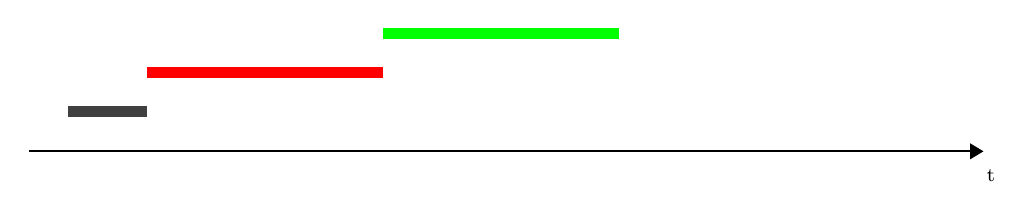
\begin{tikzpicture}
			% draw horizontal line   
			\draw[thick, -Triangle] (0,0) -- (\textwidth,0) node[font=\scriptsize,below left=3pt and -8pt]{t};
			\draw[darkgray, line width=4pt] 
			(0.5,.5) -- +(1,0);
			
			\draw[red, line width=4pt] 
			(1.5,1.0) -- +(3,0);
			
			\draw[green, line width=4pt] 
			(4.5,1.5) -- +(3,0);
	
		\end{tikzpicture}
	\end{center}
	\caption{timeline}
	\label{u}
\end{figure}

Our primary focus for optimization is the binary cut algorithm, more specifically the counting method. Its implementation in CUDA is straight forward and performance improvement are guaranteed as shown in section \TODO{add reference}. 

\subsubsection{GPU Accelerated Count Left}
We have described a CPU implementation of the countLeftService. In this section we explain how we can port this problem to the GPU. In essence we can use a general reduction as a basis version, and adapt it to sum up up elements which fulfill a certain condition, where the condition is being smaller than a given value.

Optimized reductions in CUDA are well documented and explained by the NVIDIA developer team. We make use of a reduction introduced by \TODO{Reference} and adapt it slightly to fit our needs. We will reiterate over the important optimization aspects and finally point out the specific adaptations we have made. 

We split the array of particles which are contained within one cell into smaller slices, where each slice fits one block. Then the subproblems or blocks can be run independently from each other, in other words individual blocks can be executed in parallel or also serially without any conflicts or need for block level synchronization. After running the conditional summation on each slice of the array, we end up with a an array of results. These results can then be summed together on CPU using a simple iterator. Alternatively we could invoke another sum reduction kernel for this task.

The key concepts of the reduction are:

\begin{itemize}
	\item \textbf{Leverage Shared Memory} 
	In the code depicted in figure \ref{cuda:reduction} on line 3 we invocate the shared memory, where its size is dynamic as marked with the extern keyword. In a next step (lines 10-13) we apply our condition and copy the results to shared memory. This allows us to work exclusively with shared memory, reducing the amount of costly accesses performed on global memory.
	
	\item \textbf{Increase Thread Occupancy} There exists an optimum when considering the number of operation performed by a single thread. In order to adapt the number of ops dynamically, we iterate over a certain number of elements in the global memory, as seen in figure \ref{cuda:reduction} lines 10-13. The input parameter n defines the total number of particles. Therefore if we reduce the total number of blocks by a factor of $r$, the while loop will iterate over $r$ elements. In our case we set $r$ to 32. 
	
	\item \textbf{Meta Programming} The reduction is optimized by using a template, which indicates the total number of thread per block, which is equivalent to the blockSize. Since the template is evaluated at compile time, all the if statements taking blockSize as a parameter in figure \ref{cuda:reduction} and figure \ref{cuda:reduction} do not cause any performance loss. In fact, because we are able to unroll loops, which would be evaluated at runtime, we increase the performance of the code. 

	\item \textbf{Avoid Shared Memory Bank Conflicts} In order to decrease the bank conflicts in the shared memory we want to make sure that threads in the same warp do not try to access the same memory bank. Therefore we offset each memory access by the total grid size, which is equivalent to the total number of blocks multiplied by the number of threads per block, as it can be seen on line 12 in figure \ref{cuda:reduction}.
	
	\item \textbf{Avoiding Warp Divergence} Each time we we have an control statement in the code, we introduce a divergence. On the GPU these divergences become especially bad when they are introduced inside a warp. This means that any of the threads of the 32 threads in a warp, have to execute a different code than the rest. For this reason, the $warpReduce$ method as seen in figure \ref{cuda:reduction} is introduced. We can see on line 32 in figure \ref{cuda:reduction} that this method is only executed when we reach 32 elements in the shared memory, which remain to be added together. Inside the warp reduce method, we again encounter an unrolled loop, but in this case we have no if statements that could generate a divergence. The if statements which are present, are as mentioned, evaluated at compile time only. Inside a warp we are also not dependent on synchronization, thus the thread synchronization call can be omitted as well. Note that this implementation will perform many unnecessary operations, but this does not affect the performance negatively.
	
\end{itemize}

The main difference between the proposed version and our version is that we changed the following part: 

\begin{lstlisting}[language=c++];
unsigned int i = blockIdx.x*(blockSize*2) + tid;
unsigned int gridSize = blockSize*2*gridDim.x;
sdata[tid] = 0;
while (i < n) { 
	sdata[tid] += g_idata[i] + g_idata[i+blockSize]; 
	i += gridSize; 
}
__syncthreads();
\end{lstlisting}
to:

\begin{lstlisting}[language=c++]
unsigned int i = blockIdx.x*(blockSize) + threadIdx.x;
unsigned int gridSize = blockSize*gridDim.x;
sdata[tid] = 0;

while (i < n) {
	sdata[tid] += (g_idata[i] <= cut);
	i += gridSize;
}
__syncthreads();
\end{lstlisting}

In our version we do not add up two elements with each iteration of the loop. This ensures that no memory access is attempted on global memory which is out of bounds. In the original version, if one is not careful, segmentation faults can occur on the GPU. Furthermore there are no performance penalties as we can simply increase the elements per thread if we wish to increase thread occupancy.


We execute the reduction kernel once for each cell, where we distribute the particles within the cell among a set of blocks. The number of blocks can be determined by the number of particles in this cell $n_{cell}$ divided by the number of threads per block which is set to 256 and finally we devide this further by the number of elements per thread $r$. This makes the implementation straight forward but as we increase the number of cells, we make make more calls to the reduction kernel. This is problematic because each initialization of a kernel comes with some overhead. Therefore we should come up with solution, where each kernel processes a large number of elements. As of now we have up to $d$ kernel invocation, which oftentimes reaches around 1024. There are some solutions to this problem:



\begin{figure}
	\begin{lstlisting}[language=c++]
template <unsigned int blockSize>
extern __global__ void reduce(
	float*g_idata,
	unsigned int*g_odata, 
	float cut, int n) {
	extern __shared__ int sdata[];
	
	unsigned int tid = threadIdx.x;
	unsigned int i = blockIdx.x*(blockSize) + threadIdx.x;
	unsigned int gridSize = blockSize*gridDim.x;
	sdata[tid] = 0;
	
	while (i < n) {
		sdata[tid] += (g_idata[i] <= cut);
		i += gridSize;
	}
	__syncthreads();
	
	if (blockSize >= 512) {
		if (tid < 256) {sdata[tid] += sdata[tid + 256];}
		__syncthreads();
	}
	if (blockSize >= 256) {
		if (tid < 128) {sdata[tid] += sdata[tid + 128];}
		 __syncthreads();
	}
	if (blockSize >= 128) {
		if (tid < 64) {sdata[tid] += sdata[tid + 64];}
		 __syncthreads();
	}
	if (tid < 32) {
		warpReduce<blockSize>(sdata, tid);
	}
	if (tid == 0) {
		g_odata[blockIdx.x] = sdata[0];
	}
}

template <unsigned int blockSize>
extern __device__ void warpReduce(
volatile int *sdata, unsigned int tid) {
	if (blockSize >= 64) sdata[tid] += sdata[tid + 32];
	if (blockSize >= 32) sdata[tid] += sdata[tid + 16];
	if (blockSize >= 16) sdata[tid] += sdata[tid + 8];
	if (blockSize >= 8) sdata[tid] += sdata[tid + 4];
	if (blockSize >= 4) sdata[tid] += sdata[tid + 2];
	if (blockSize >= 2) sdata[tid] += sdata[tid + 1];
}
	\end{lstlisting}
	\label{cuda:reduction}
\end{figure}


\begin{itemize}
	\item \textbf{Single Kernel with Cell ID} We can build a reduction kernel where we take an additional array in global GPU memory as an input. The additional array has the same size as the particle position array, but it stores the cellID for each particle. Furthermore we increase the shared memory size to the product of the number of threads per block by the total number of cells which are currently being iterated over. This allows us perform the summation and store its results in the correct place in the shared memory. This version however, requires a very large shared memory, thus forcing us to reduce the number of threads per block. Furthermore we have to store another array for the cellID on the GPU. 
	\item \textbf{Block Padding} Another solution would be to introduce a padding with a constant value of 0 after each slice of particles which are contained within one cell. This padding range starts with the last particle within the cell and ends with the last array index which is still contained within the same block. Therefore we only need to keep track of which block processes which cell and are able to reconstruct the actual counts for each cell. We need to increase the array which stores the particle positions by a maximum of threads per kernel times the maximum number of items per thread times $d$. In a normal setup only a fraction of the total memory size needed. However it requires us correctly load \TODO{continue}
\end{itemize}


\subsubsection{GPU Accelerated Partitioning}

The main bottlenecks of the orb algorithm are now the data transfer between the CPU and GPU and the partitioning of the data. Both problems can be resolved by partitioning the array on the GPU directly thus also removing the need to transfer the data back and forth between the CPU and the GPU.

We describe measurements which were done using the reduction in CUDA, we mention how the reduction cannot necessarily be improved a lot and that the data transfer between the GPU and CPU is the main bottleneck now. We mention how building the tree on the does not make a lot of sense. We explain why instead we focus our efforts to implement a GPU reshuffling method, which can improve runtime by reducing the reshuffling costs and also remove CPU GPU transfers between invocations of the binary cut algorithm altogether. 

We add a timeline which is based on measurements with a CUDA enhanced binary cut algorithm. 
\begin{figure}[H]
	\begin{center}
		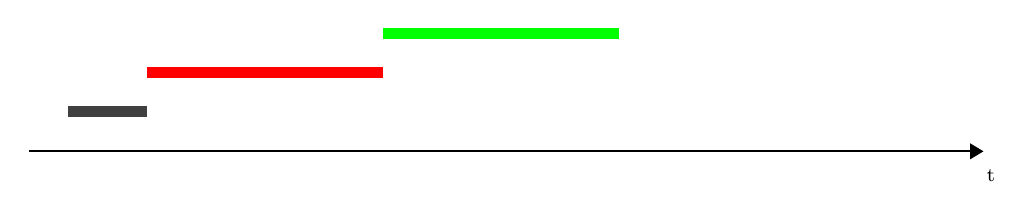
\begin{tikzpicture}
			% draw horizontal line   
			\draw[thick, -Triangle] (0,0) -- (\textwidth,0) node[font=\scriptsize,below left=3pt and -8pt]{t};
			\draw[darkgray, line width=4pt] 
			(0.5,.5) -- +(1,0);
			
			\draw[red, line width=4pt] 
			(1.5,1.0) -- +(3,0);
			
			\draw[green, line width=4pt] 
			(4.5,1.5) -- +(3,0);
			
		\end{tikzpicture}
	\end{center}
	\caption{timeline}
	\label{u}
\end{figure}

The partitioning algorithm is a widely used concept and there are various implementations used in different variants of the quick-sort algorithm. The overall design of the implementation is guided by \TODO{Insert ref} and the scan is taken from GPU Gems \TODO{Insert ref}. The main and probably only disadvantage of partitioning the particle array on the GPU, is that it cannot be done in place, thus we need another temporary array allocated on the GPU memory which further restricts the total number of particles. Furthermore we need to store the permutations, because we need to apply them to the other axes as well. We could as well simply perform all permutations from the same kernel at the same time, but this would require 3 temporary arrays, thus reducing the total number of particles by a factor of 2. The solution with the partition array and a single temporary array only results in a reduction of the particles by a factor of $\frac{5}{3}$. 	

\begin{itemize}
	\item As we increase the number of cells, we make more calls to the reduction kernel 
	
\end{itemize}

\begin{figure}[H]
	
\begin{lstlisting}[language=c++]
template <unsigned int blockSize>
__global__ void partition(
unsigned int * g_offsetLessEquals,
unsigned int * g_offsetGreater,
float * g_idata,
float * g_odata,
unsigned int * g_permutations,
float pivot,
unsigned int nLeft,
unsigned int n) {
	__shared__ unsigned int s_lessEquals[blockSize * 2];
	__shared__ unsigned int s_greater[blockSize * 2];
	__shared__ unsigned int s_offsetLessEquals;
	__shared__ unsigned int s_offsetGreater;
	
	unsigned int tid = threadIdx.x;
	
	unsigned int i = blockIdx.x * blockSize * 2 + 2 * tid;
	unsigned int j = blockIdx.x * blockSize * 2 + 2 * tid + 1;
	
	bool f1, f2, f3, f4;
	if (i < n) {
		f1 = g_idata[i] <= pivot; f2 = not f1;
		s_lessEquals[2*tid] = f1;
		s_greater[2*tid] = f2;
	} else {
		f1 = false; f2 = false;
		s_lessEquals[2*tid] = 0;
		s_greater[2*tid] = 0;
	}
	
	if (j < n) {
		f3 = g_idata[j] <= pivot; f4 = not f3;
		s_lessEquals[2*tid+1] = f3;
		s_greater[2*tid+1] = f4;
	} else {
		f3 = false; f4 = false;
		s_lessEquals[2*tid+1] = 0;
		s_greater[2*tid+1] = 0;
	}
	
	__syncthreads();
	
	scan(s_lessEquals, tid, blockSize * 2 );
	scan(s_greater, tid, blockSize * 2);
	\end{lstlisting}
	\caption{Partitioning kernel I}
	\label{cuda:partitionI}
\end{figure}



\begin{figure}
\begin{lstlisting}[language=c++]
	
	__syncthreads();
	
	if (tid == blockSize - 1) {
		s_offsetLessEquals = 
		atomicAdd(g_offsetLessEquals, s_lessEquals[blockSize*2-1] + f3);
		s_offsetGreater = 
		atomicAdd(g_offsetGreater, s_greater[blockSize*2-1] + f4);
	}
	
	__syncthreads();
	
	unsigned int indexA = (s_lessEquals[2*tid] + s_offsetLessEquals) * f1 +
	(s_greater[2*tid] + s_offsetGreater + nLeft) * f2;
	
	unsigned int indexB = (s_lessEquals[2*tid+1] + s_offsetLessEquals) * f3 +
	(s_greater[2*tid+1] + s_offsetGreater + nLeft) * f4;
	
	if (i < n) {
		g_odata[indexA] = g_idata[i];
		g_permutations[i] = indexA;
	}
	
	if (j < n) {
		g_odata[indexB] = g_idata[j];
		g_permutations[j] = indexB;
	}
}
	\end{lstlisting}
	\caption{Partitioning kernel II}
	\label{cuda:partitionII]}
\end{figure}


\begin{figure}[H]
	\begin{lstlisting}[language=c++]
__device__ void scan(volatile unsigned int * s_idata, unsigned int thid, unsigned int n) {
	unsigned int offset = 1;
	for (unsigned int d = n>>1; d > 0; d >>= 1) // build sum in place up the tree
	{
		__syncthreads();
		if (thid < d)
		{
			unsigned int ai = offset*(2*thid+1)-1;
			unsigned int bi = offset*(2*thid+2)-1;
			s_idata[bi] += s_idata[ai];
		}
		offset *= 2;
	}
	if (thid == 0) { s_idata[n - 1] = 0; } // clear the last element
	for (unsigned int d = 1; d < n; d *= 2) // traverse down tree & build scan
	{
		offset >>= 1;
		__syncthreads();
		if (thid < d)
		{
			unsigned int ai = offset*(2*thid+1)-1;
			unsigned int bi = offset*(2*thid+2)-1;
			unsigned int t = s_idata[ai];
			s_idata[ai] = s_idata[bi];
			s_idata[bi] += t;
		}
	}
}
	\end{lstlisting}
	\caption{Device Scan Kernel}
	\label{cuda:scan}
\end{figure}



\begin{figure}[H]
	\begin{lstlisting}[language=c++]
template <unsigned int blockSize>
__global__ void permute(
float * g_idata,
float * g_odata,
unsigned int * g_permutations,
int n) {
	unsigned int tid = threadIdx.x;
	
	unsigned int i = blockIdx.x * blockSize * 2 + 2 * tid;
	unsigned int j = blockIdx.x * blockSize * 2 + 2 * tid + 1;
	//unsigned int gridSize = blockSize*2*gridDim.x;
	
	if (i < n) {
		g_odata[g_permutations[i]] = g_idata[i];
	}
	
	if (j < n) {
		g_odata[g_permutations[j]] = g_idata[j];
	}
}
	\end{lstlisting}
	\caption{Device Permute Kernel}
	\label{cuda:permute}
\end{figure}



\subsubsection{Memory allocation}

We can use several strategies in order to improve the performance of memory allocation: 

\begin{enumerate}
	\item \textbf{Pinned Memory} As the GPU cannot access the default paged memory directly, when copying memory from the host to the device, the memory must first be copied to pinned memory. This means if we use pinned memory directly with $cudaMallocHost()$, data transfers can be around twice as fast. In our implementation we use pinned memory for all data, which need to be either sent from the host to device or vice versa.
	\item \textbf{Reuse Memory} We can avoid allocation and freeing commands altogether and instead reuse previously allocated memory whenever possible. In our implementation we allocate the memory in the very beginning, whereas we have a fixed number of particles and a fixed upper limit for the number of cells. This is true for both the CPU and GPU memory.
\end{enumerate}

We limit memory allocation and freeing to the very beginning and end of the orb algorithm. This reduces the runtime of the algorithm by a substantial factor. Furthermore we use pinned memory

\subsubsection{Data Transfer}

We can use several strategies in order to improve the performance of data transfers: 

\begin{enumerate}
	\item \textbf{Reuse Data} We can avoid data transfers, by writing kernels out of code which was done on the CPU before. In our case we send the particle data from the host to device once
	\item \textbf{Reduce Data} We can reduce the total number of data, which needs to be sent to the GPU. We do this 
	\item \textbf{CUDA Streams} 
	\item \textbf{Data Batches}
	
\end{enumerate}

Most importantly we try to reduce the overhead generated 

\subsubsection{CUDA streams}

Cuda streams can be leveraged to improve the performance of data-intensive applications by allowing different tasks to be executed in parallel on the GPU. This can be used to overlap data transfers with computation, or to execute multiple kernels concurrently. Some GPU's have several Kernel engines, this means that the execution of kernel code can be overlapped when 
\newpage

\subsection{Integration into PKDGRAV}



\newpage
\section{Performance Analysis of ORB}

We will use two system for our performance analysis. One is the Summit supercomputer which has been described in section 3.1. The other has the following specs:


AMD EPYC 7702 64-Core Processor, Tesla T4.


\subsection{Methodology}

\subsection{Results}


\begin{comment}
	\begin{figure}[H]
		\begin{center}
			\begin{tikzpicture}
				\begin{axis}[
					height=10cm,width=13cm, 
					title={Measured Performance with $d = 1024$},
					xlabel={Particle Count},
					ylabel={Execution Time (ms)},
					]
					
					\foreach \i in {0,...,3}{
						\pgfmathsetmacro\suffix{int(pow(2,\i))};
						
						\addplot +[] 
						table [col sep=comma, x=N, y=time] 
						{../../code/out/measurements\suffix.csv};
						
						\addlegendentryexpanded{\# $\suffix$};
						
					}	
				\end{axis}
			\end{tikzpicture}
		\end{center}
	\end{figure}
\end{comment}


\subsection{Comparison to Theoretical Model}


\subsection{Conclusion}


% Use for reduction explanation https://texample.net/tikz/examples/database-decimation-process/
\bibliographystyle{unsrt}
\bibliography{reference}

\end{document}
